\documentclass[tcc]{ic}

\hypersetup{
    colorlinks = {true},
    linktocpage = {false},
    plainpages = {false},
    linkcolor = {Blue},
    citecolor = {Blue},
    urlcolor = {Red},
    unicode = {true},
    pdftitle = {Título do trabalho}, 
    pdfauthor = {Fulano da Silva Alves},
    pdfsubject = {Proposta de Dissertação de Mestrado},
    pdfkeywords = {processamento gráfico, imagens médicas, visão computacional, aprendizagem profunda, aumento de dados, graphics processing, medical images, computer vision, deep learning, data augmentation}
}

\usepackage{algorithm}
\usepackage{algpseudocode}
\usepackage{enumerate}
\usepackage{fancyhdr}
\usepackage{acronym}
\usepackage{natbib}
\usepackage{lipsum}  
\usepackage{amsmath}

\makeatletter
\renewcommand{\ALG@name}{Algoritmo}
\renewcommand{\listalgorithmname}{List of \ALG@name s}
\makeatother

\newcolumntype{Y}{>{\centering\arraybackslash}X}

\begin{document}

    % Inclui o preâmbulo do documento (Informações da capa e contracapa)
    % author: Matheus T. dos Santos
% co-authors:
%   - Claude (claude-opus-4-8), 2026-08-13 -- formatacao mecanica autorizada por Matheus
%     (suspensao pontual da Regra 3): italico em "data races" no titulo (capa/folha de rosto).
%     Nenhuma outra alteracao.
\titulo{Mapeando o custo e a fronteira de segurança do Rust no território de \textit{data races} em algoritmos de controle}

\autor{Matheus Tenório dos Santos}{mtds@ic.ufal.br}{https://github.com/matheuswhite}

\orientador{Ícaro Bezerra Queiroz de Araújo}{icaro@ic.ufal.br}{Instituto de Computação}{Universidade Federal de Alagoas}{}

 \examinador{Allan de Medeiros Martins}{allan@dee.ufrn.br}{Departamento de Engenharia Elétrica}{Universidade Federal do Rio Grande do Norte}{}

 \examinadorDois{Glauber Rodrigues Leite}{glauber@ic.ufal.br}{Instituto de Computação}{Universidade Federal de Alagoas}{}

\dataMesAno{Agosto}{2026}{}


    \selectlanguage{portuguese}
    
    % Capa, contracapa e avaliadores
    \capa
    
    % Agradecimentos
    \begin{agradecimentos}

Agradeço primeiramente a Jesus por me sustentar nesta jornada, pois sem Ele nada seria. Agradeço à minha noiva, Ana Clara Rocha Albuquerque Lima, por me incentivar a continuar e me dar apoio nos momentos mais difíceis. Agradeço aos meus pais, Marta Maria Tenório dos Santos e Robson dos Santos, por me lembrarem que o equilíbrio e a constância são importantes. Agradeço ao meu orientador, Ícaro Bezerra Queiroz de Araújo, pelo direcionamento do trabalho e pelo auxílio nos momentos de dúvidas. Agradeço aos membros da banca, por se disporem a ler esta dissertação e por contribuírem na sua melhoria. Agradeço ao instituto de inovação EDGE por todo o suporte, ferramentas e flexibilidade ofertados para que eu me dedicasse à construção desta pesquisa. Agradeço também aos meus colegas de trabalho por sempre estarem dispostos a discutir melhorias e pelos conselhos textuais.

\end{agradecimentos}

    
    % Resumo e Abstract
    % author: Matheus T. dos Santos
% co-authors:
%   - Claude (claude-opus-4-8), 2026-08-13 -- formatacao mecanica autorizada por Matheus
%     (suspensao pontual da Regra 3): italico em estrangeirismos (todas as ocorrencias) no
%     corpo do resumo. Siglas nao convertidas para \ac{} (o resumo precede a Lista de Siglas).
%     Nenhuma palavra do texto foi alterada.
\begin{resumo}

Em controle digital de malha fechada, não cumprir o requisito de tempo do período de amostragem pode desestabilizar o sistema por completo, causando acidentes graves. A natureza do controle digital exige estados compartilhados: seja na aquisição de dados, seja na alteração de parâmetros feita pelo usuário, seja na atuação do sinal de controle. Os estados compartilhados acessados por diversos contextos, onde pelo menos um deles realiza uma escrita e pelo menos um acesso é não sincronizado, levam a um \textit{data race}. O estado da arte hoje na implementação de controle digital, em sistemas embarcados, envolve C+MISRA+Sanitizers para evitar \textit{data races}. Entretanto este método depende da disciplina do desenvolvedor e de detectar \textit{data races} exercitados em tempo de execução. Com a linguagem Rust, essas garantias são movidas do desenvolvedor para o compilador e os \textit{data races} não são mais detectados em tempo de execução, mas sim eliminados em tempo de compilação, através do sistema de tipos do Rust (\textit{Send}/\textit{Sync} e \textit{borrow checker}). Todavia, o Rust exige uma sincronização forçada a qual possui um custo. Também é desconhecido quais resquícios de \textit{unsafe} ainda permanecem no Rust. Deste modo, qual a fronteira entre \textit{safe} e \textit{unsafe} nos padrões de \textit{data race}, no domínio de algoritmos embarcados de controle, e qual o custo das garantias do Rust? Neste trabalho, é proposta uma taxonomia para classificar os padrões de \textit{data race} presentes nos algoritmos de controle. Após isso, a fronteira entre \textit{safe} e \textit{unsafe} nestes padrões é caracterizada. Além disso, é catalogado o espaço de design das garantias que tornam o \textit{data race} inexprimível. Também é construído o veículo de experimentos: Aule, uma biblioteca de controle construída para instanciar os algoritmos de controle utilizados nos experimentos. Atualmente, Aule contém a base principal para a construção dos experimentos em uma planta física, com os blocos de sincronização em desenvolvimento. Também está presente neste trabalho um panorama comparativo do ecossistema \textit{open-source} do Rust para bibliotecas de controle. Por fim, é mostrado neste trabalho um caso demonstrativo de recusa do compilador Rust \textit{safe}, quando o código possui \textit{data race}.

\palavrasChave{\textit{Data race}; Segurança de Memória; Sistemas de Controle; Rust; Sistemas Embarcados}

\end{resumo}

    \begin{abstract}

In closed-loop digital control, failing to meet the time requirement of the control period (missing the deadline) could destabilize the entire system, causing severe accidents. The nature of digital control requires shared states: in data acquisition, in user parametrization, or in control signal output. The shared states accessed by multiple contexts, in which at least one of them performs a write and at least one of them is not synchronized, lead to a data race. In code with a data race, the behavior is undefined, causing digital control to miss deadlines. The current state of the art in digital control implementation, in embedded systems, relies on C+MISRA+Sanitizers to avoid data races. However, this method depends on the developer's discipline and on detecting data races exercised at runtime. With the Rust programming language, these guarantees are moved from the developer to the compiler and the data races are not detected at runtime anymore, but they are eliminated at compile time, using Rust's type system (Send/Sync and borrow checker). However, Rust needs a forced synchronization, which has a cost. It is also unknown which residual unsafe remains in Rust. Thus, what is the boundary between safe and unsafe in data race patterns, in the domain of embedded control algorithms, and what is the cost of Rust's guarantees? In this work, a taxonomy is proposed to classify the data race patterns within the control algorithms. Furthermore, the guarantee design space that makes data races unrepresentable is cataloged. The experiment vehicle is built: Aule, a control library designed to instantiate the control algorithms used in the experiments. Currently, Aule provides the foundation for building the experiments on a physical plant (an inverted pendulum), with the synchronization blocks under development. A comparative overview of Rust's open-source ecosystem for control libraries is shown. Finally, this work shows a demonstrative case of Rust's safe compiler refusal, when the code contains a data race.

\keywords{Data race; Memory Safety; Control Systems; Rust; Embedded Systems}
\end{abstract}

    \renewcommand{\headrulewidth}{0pt}
\listoftables

    \listoffigures
%\ref{fig:nome_rotulo}

    



    % author: Matheus T. dos Santos
% co-authors:
%   - Claude (claude-opus-5), 2026-08-03 -- preenchimento da lista com as siglas levantadas
%     no texto dos capitulos 1, 3, 4 e 5; removidas as 11 siglas herdadas do template
%     (BCC, CCR, CRS, VRS, CVLI, DEA, DMUs, SSP, CISPs, NEAC, DETRAN), que pertencem a
%     outro trabalho. Autorizado por Matheus nesta data.
\chapter*{Lista de Siglas}

\begin{acronym}[TOCTOU]
    \acro{ADC}{\textit{Analog-to-Digital Converter}}
    \acro{API}{\textit{Application Programming Interface}}
    \acro{ASan}{\textit{Address Sanitizer}}
    \acro{CAS}{\textit{Compare-And-Swap}}
    \acro{CI}{\textit{Continuous Integration}}
    \acro{CPU}{\textit{Central Processing Unit}}
    \acro{CSV}{\textit{Comma-Separated Values}}
    \acro{DMA}{\textit{Direct Memory Access}}
    \acro{EDO}{Equação Diferencial Ordinária}
    \acro{FFI}{\textit{Foreign Function Interface}}
    \acro{GPIO}{\textit{General Purpose Input/Output}}
    \acro{HAL}{\textit{Hardware Abstraction Layer}}
    \acro{HiL}{\textit{Hardware-in-the-Loop}}
    \acro{IAE}{\textit{Integral of Absolute Error}}
    \acro{IHM}{Interface Homem-Máquina}
    \acro{IRQ}{\textit{Interrupt Request}}
    \acro{ISA}{\textit{Instruction Set Architecture}}
    \acro{ISE}{\textit{Integral of Squared Error}}
    \acro{ISO}{\textit{International Organization for Standardization}}
    \acro{ISR}{\textit{Interrupt Service Routine}}
    \acro{ITAE}{\textit{Integral of Time-weighted Absolute Error}}
    \acro{LoC}{Linhas de Código}
    \acro{LTI}{\textit{Linear Time-Invariant}}
    \acro{MCU}{\textit{Microcontroller Unit}}
    \acro{MISRA}{\textit{Motor Industry Software Reliability Association}}
    \acro{ODE}{\textit{Ordinary Differential Equation}}
    \acro{OOB}{\textit{Out-of-Bounds}}
    \acro{OS}{\textit{Operating System}}
    \acro{PAC}{\textit{Peripheral Access Crate}}
    \acro{PID}{\textit{Proportional-Integral-Derivative}}
    \acro{PWM}{\textit{Pulse Width Modulation}}
    \acro{RAM}{\textit{Random Access Memory}}
    \acro{RISC}{\textit{Reduced Instruction Set Computer}}
    \acro{RK4}{Runge-Kutta de quarta ordem}
    \acro{RMW}{\textit{Read-Modify-Write}}
    \acro{RTIC}{\textit{Real-Time Interrupt-driven Concurrency}}
    \acro{RTOS}{\textit{Real-Time Operating System}}
    \acro{SDK}{\textit{Software Development Kit}}
    \acro{SISO}{\textit{Single-Input Single-Output}}
    \acro{SoC}{\textit{System on Chip}}
    \acro{SPI}{\textit{Serial Peripheral Interface}}
    \acro{SPSC}{\textit{Single-Producer Single-Consumer}}
    \acro{SS}{\textit{State Space}}
    \acro{SWD}{\textit{Serial Wire Debug}}
    \acro{TF}{\textit{Transfer Function}}
    \acro{TOCTOU}{\textit{Time-of-check-Time-of-use}}
    \acro{TSan}{\textit{Thread Sanitizer}}
    \acro{UART}{\textit{Universal Asynchronous Receiver/Transmitter}}
    \acro{UB}{\textit{Undefined Behaviour}}
    \acro{UBSan}{\textit{Undefined Behavior Sanitizer}}
\end{acronym}

 
    
    % Sumário
    \tableofcontents
    \thispagestyle{empty}
    
    % Início dos capítulos
    \inicio
    
    % author: Matheus T. dos Santos
% co-authors:
%   - Claude (claude-opus-5), 2026-08-03 -- revisao mecanica autorizada por Matheus nesta data:
%     ortografia/acentuacao, concordancia, pontuacao, aspas LaTeX (``''), labels/refs invalidos
%     e unificacao \cite -> \citep. Nenhum conteudo, argumento ou frase autoral foi reescrito.
%   - Claude (claude-opus-4-8), 2026-08-07 -- padronizacao de genero de HAL (feminino)
%     autorizada por Matheus nesta data (suspensao pontual da Regra 3). Nenhum conteudo
%     ou frase autoral foi alterado.
%   - Claude (claude-opus-5), 2026-08-10 -- troca de chave de citacao autorizada por Matheus
%     nesta data (suspensao pontual da Regra 3): \citep{book:deadline-requirement} ->
%     \citep{article:liu-layland-hard-real-time} na secao 1.1, por falta de acesso ao livro do
%     Buttazzo. Somente a chave mudou; nenhuma palavra do texto foi tocada.
\mychapter{Introdução}{cap:introducao}

\section{Contextualização}

Máquinas que necessitam de controle automático são uma grande inovação da modernidade. Essas máquinas estão presentes não só em fábricas e indústrias, como motores e bombas, como também nos produtos mais sutis, como um marca-passo para sincronizar as batidas do coração. Controlar essas máquinas indica executar algum processo para que elas sigam da melhor forma um valor de referência. Isso pode ser feito de maneira analógica ou digital. Com a diminuição de custo e popularização da computação, utilizar a teoria de controle \citep{book:ogata} em computadores, na forma de programas (ou algoritmos), se tornou cada vez mais viável e desejado. Além disso, o desenvolvimento e evolução de processadores \ac{RISC}, como ARM e RISC-V, permitiram um avanço ainda maior na implantação destes algoritmos de controle em dispositivos mais baratos e com periféricos para interagir com o mundo exterior. Esses dispositivos são os \ac{SoC}: processadores com periféricos para interagir com o meio externo, como: \ac{GPIO}, \ac{UART}, \ac{SPI}, etc. Um tipo de \ac{SoC} é uma \ac{MCU}, na qual está contido o core (processador), a memória e os periféricos. É importante os microcontroladores possuírem periféricos de interação com o mundo exterior, pois os algoritmos de controle executam em malha fechada. Isso quer dizer que o algoritmo envia sinais e recebe sinais como resposta ao estado da planta que ele está controlando. Esse controle deve ser feito em um período fixo e o tempo máximo para atuar em cada ciclo é chamado de deadline. Perder deadline aqui é diferente de perder deadline em um Desktop e a interface gráfica travar. Perder deadline aqui é o risco de o sistema controlado se desestabilizar e causar prejuízos. Não só financeiros, como uma planta de uma fábrica parada, mas também pessoais, podendo um motor instável causar acidentes ou um marca-passo causar uma arritmia \citep{article:liu-layland-hard-real-time}.

Note que, no algoritmo de controle, o usuário pode definir a referência e isso chega para o algoritmo de controle de forma assíncrona. A tarefa de controle, por ser crítica e não poder perder deadline, é executada em uma tarefa dedicada, enquanto a interação com o usuário (uma \ac{IHM}, por exemplo), por ser de baixa prioridade, está em outra tarefa. Além disso, ainda existe a aquisição de dados (a resposta do estado do mundo exterior), obtida via interrupção. Ou seja, sempre que um novo dado está disponível, a \ac{MCU} é interrompida pelo periférico e este salva o valor lido dos sensores. Note que existem dois contextos fora da tarefa principal que contém o algoritmo de controle. E esses dois contextos precisam comunicar suas atualizações para a tarefa principal. Desta forma, existem estados que mais de um contexto precisa utilizar (ou para atualizar, ou para ser lido e utilizado) e acessar esses dados concorrentemente, sem sincronização, gera um data race. Perceba que é da natureza da aplicação possuir esses estados compartilhados e não um erro do programador.

O microcontrolador (ou \ac{SoC}) é barato por um motivo bem direto: ele possui recursos bem limitados. Apenas o necessário para fazer uma tarefa específica, que neste caso é controlar uma planta. Algumas centenas de kilobytes de memória e algumas centenas de MHz de processamento já são o suficiente para essa tarefa. Utilizar os gigabytes de memória e os GHz de configurações desktops seria gastar dinheiro a mais, pois uma configuração com menos recurso já resolve o problema. Para esse sistema com poucos recursos é fundamental utilizar uma linguagem que, além de permitir a gerência desses recursos, também permita que estes não sejam desperdiçados. Com isso, uma das linguagens que se encaixam neste requisito é a linguagem C. É nesta linguagem que as \acp{HAL} dos microcontroladores são construídas. Por ser uma linguagem utilizada desde a década de 70, ela possui uma abundância de código legado. Possuir o poder de gerenciar os recursos (como memória) é uma grande responsabilidade, e se não utilizado do jeito correto pode gerar problemas, tal como não sincronizar o acesso concorrente a um dado e gerar data races. Com isso, um padrão foi criado para diminuir os erros cometidos pelo desenvolvedor, o padrão \ac{MISRA} \citep{doc:MISRA}. Se o desenvolvedor seguir esse padrão, o seu código vai estar menos propenso aos erros citados. Porém, a própria frase denuncia o problema: ``\textbf{Se} o desenvolvedor seguir...''. Se o desenvolvedor não seguir, o problema continua lá. O \ac{MISRA} é apenas uma convenção, não impede a compilação de um programa com problemas. Além disso, a análise estática que verifica se o padrão \ac{MISRA} está sendo seguido não é completa. Para contornar isso, é utilizado um sanitizer \citep{doc:TSan}. Com o sanitizer é possível executar o programa e capturar problemas, como data races. Entretanto, os sanitizers apenas minimizam o problema, pois surgem outros com ele, pois: a cobertura é dinâmica, visto que só o que é exercitado durante a execução do programa é pego pelo sanitizer. Se um data race existir e o programa não executar aquele trecho, o sanitizer não o pega. Outro ponto é sua execução, pois: alguns sanitizers, como o \ac{TSan}, não executam em ambiente embarcado, apenas no desktop; e cada sanitizer identifica um tipo de bug, sendo necessário executar uma vez para cada tipo de sanitizer. O sanitizer apenas detecta o bug que foi exercitado, ele não previne qualquer bug daquela classe. Deste modo, a garantia hoje para sistemas de controle depende da disciplina do desenvolvedor e de o bug ter sido exercitado. Bugs latentes no código não são detectados e vão para a produção causando danos à planta controlada.

Uma linguagem mais recente, chamada Rust, desloca a garantia de detecção em tempo de execução para a recusa em tempo de compilação, através dos mecanismos: Send/Sync e borrow checker \citep{article:rust-safe-soundness} e \citep{article:rust-critical}. Além de mover a garantia, essa linguagem ainda mantém as funcionalidades de: controle sobre recursos (como memória) e baixa utilização de recursos. Apesar de ser uma linguagem recente, quando comparada com a linguagem C, ela já possui mais de 10 anos. A proposta de utilizá-la em algoritmos embarcados de controle somente agora se deve ao ecossistema de sistemas embarcados, da linguagem Rust, estar maduro recentemente, por exemplo: a maturidade do no\_std (bare-metal) da ESP32 ter ocorrido somente por volta de 2025 \citep{url:esp-rust-no-std-stable}. A linguagem não oferece uma bala de prata, visto que existem custos e incógnitas associados a mover a garantia: não saber onde os resquícios de unsafe (código fora das garantias da linguagem) se encontram nos padrões de data races e forçar sincronização. Essa sincronização tem um custo e esse custo pode afetar, ou não, deadlines em malhas rápidas, causando danos como em motores instáveis e em marca-passos fora do ritmo. Para investigar o custo das garantias de sincronização é necessário um veículo que permita a implementação de data races em algoritmos de controle realistas. Entretanto, o ecossistema Rust de controle não possui tal veículo que reúne suporte a: sistemas embarcados (no\_std), tratamento de concorrência e genérico pleno (\ref{sec:control-repos}). Com isso, a biblioteca Aule \citep{aule} foi construída, para ser veículo desta investigação.

Com essas lacunas apontadas, a pergunta que surge sobre utilizar Rust em algoritmos embarcados de controle é: onde se encontra a fronteira entre safe e unsafe do Rust em data races, no domínio de algoritmos embarcados de controle? Respondida a pergunta anterior, qual o custo cobrado pelas garantias da linguagem sobre data races?

\section{Objetivos}

\subsection{Objetivo Geral}

O objetivo geral é caracterizar a fronteira entre safe e unsafe dos data races presentes em algoritmos de controle que compartilham estado entre múltiplos contextos e avaliar o custo para implementar a sincronização imposta pelo lado safe da fronteira.

\subsection{Objetivos Específicos}

Os objetivos 1, 2 e 3 estão desenvolvidos na qualificação, enquanto os objetivos 4, 5, 6, 7 e 8 serão desenvolvidos na pós-qualificação.

\begin{enumerate}
\item Propor uma taxonomia de padrões de data races presentes em algoritmos de controle que compartilham estado entre múltiplos contextos;
\item Caracterizar a fronteira entre safe e unsafe destes padrões de data races;
\item Catalogar o espaço de design de implementar as garantias impostas para tornar os data races, presentes no lado safe da fronteira, inexprimíveis;
\end{enumerate}

\begin{enumerate}
\setcounter{enumi}{3}
\item Implementar, na biblioteca Aule, um subconjunto das garantias (um por eixo do espaço de design) impostas para tornar os data races, presentes no lado safe da fronteira, inexprimíveis;
\item Avaliar o overhead de tempo de execução destas implementações (em Rust) e em implementações em C, em controladores com realimentação de estados, em controle de um pêndulo invertido, em placas com ESP32 (Xtensa);
\item Avaliar a perda de deadlines nos algoritmos de controle implementados em Rust e em C;
\item Comparar o overhead de tempo de execução e a perda de deadlines entre a implementação em Rust e em C de controladores que compartilham estado entre múltiplos contextos;
\item Comparar a verificação em tipos do Rust, que torna os data races inexprimíveis, e o estado da arte em C+\allowbreak MISRA+\allowbreak sanitizers, que detecta os data races em tempo de execução.
\end{enumerate}

\section{Visão Geral da Qualificação}

Dado que a proposta está descrita, o restante é organizado assim: no capítulo \ref{cap:fundamentacao} está presente a fundamentação com as explicações e definições de data race e garantias do Rust. É neste capítulo que existe o conhecimento necessário para a compreensão do resto do texto. Na metodologia, capítulo \ref{cap:metodologia}, está presente a taxonomia, a fronteira entre safe e unsafe e o catálogo do espaço de design. No capítulo a seguir (\ref{cap:resultados}), são descritos os resultados parciais: o estado atual da biblioteca Aule; o caso demonstrativo P1; e o panorama do ecossistema open-source do Rust, para bibliotecas de controle. Por fim, no capítulo \ref{cap:cronograma} está descrito o cronograma pós-qualificação.

Na qualificação, os objetivos de 1 a 3 estão concluídos, enquanto os objetivos de 4 a 8 serão concluídos na dissertação. Nos resultados parciais está a evidência já colhida. A ordem dos capítulos é construída para facilitar o entendimento, pois se começa com a pergunta, levando para os objetivos do trabalho. Após isso são apresentados os fundamentos necessários para o entendimento geral, seguido do método utilizado para coletar e verificar as evidências, fechando com o cronograma do que será realizado após este trabalho.

    \mychapter{Trabalhos Relacionados}{cap:relatedworks} 

    % 3
\mychapter{Fundamentação teórica}{cap:fundamentacao}

% 3.3
\section{Concorrência e Modelo de Memória}

% 3.3.1
\subsection{Contextos de execução concorrente}
\label{subsec:contexts}

Quando um controlador, embarcado em um microcontrolador, está atuando em uma planta física existem três fluxos ocorrendo de forma concorrente: primeiro a aquisiçao do estado da planta, pois o controlador precisa conhecer o estado atual do mundo físico, antes de atuar nele; após isso, é realizado o calculo do sinal de controle, a partir dos dados de aquisição e estados internos; e por último o sinal de controle gerado é enviado para o mundo físico através de atuadores. Cada um desses fluxos é executado em um contexto diferente dentro do microcontrolador: A aquisição de dados pode utilizar dois contextos diferentes, a ISR e a DMA, enquanto o cálculo é feito majoritariamente em tarefas no microcontrolador. Uma ISR é uma rotina que trata uma interrupção, pois quando o dado da aquisição está pronto, o periférico que le este dado (por exemplo um ADC), interrompe a MCU para este dado ser armazenado na memória do microcontrolador \citep{book:lee-seshia}. Enquanto isso, a DMA serve para transferir dados de diferentes regiões da memória, sem a intervenção da MCU \citep{book:stallings}, isso alivia a carga da MCU para realizar outras ações, como realizar os calculo do próximo sinal de controle. Esses fluxos ocorrem com concorrencia entre os tipos de fluxos (ISR/DMA x Tarefa). Com esses vários fluxos ocorrendo concorrentemente, surge dois problemas: como os dados do fluxo de acquição são enviados para o fluxo de calculo do sinal de controle? E como o sinal de controle, calculado no fluxo de calculo, é enviado para o fluxo de atuação? Esses dois problemas fazem parte da mesma categoria de problemas: sincronização de memória entre fluxos de execução.

Cada fluxo anterior pode ser mapeado em um ou mais contexto e cada contexto possui suas características e restrições. A ISR é capaz de executar código e interrompe outro contexto para ser executada (preempção), entretanto a sincronização de uma região de memória compartilhada não pode ser bloqueante, pois existiria um deadlock. Este deadlock ocorre pois a ISR ficar bloqueada (ou dormindo) esperando a tarefa, que ela mesmo preemptou, desbloquear a condição nunca vai acontecer, pois a tarefa deve esperar a ISR terminar, ficando em um loop de espera infinito. A DMA possui também características e restrições peculiares, pois não é capaz de executar código, dado que ela apenas move dados de uma região de memória para outra região. Por esse motivo, não existe bloqueio relacionada a ela, pois não executa código; e também é assincrona com relação a tarefa, pois ela é independente da MCU, por definição. E por último, tem-se a tarefa, possuindo o menor nível de restrições, pois é capaz de executar código e pode ser bloqueada na sincronização da região de memória. Sua relação com outras tarefas, depende do escalonador, podendo ser preempitivo (interrompendo outras tarefas para executar) ou cooperativo (só executa quando a outra tarefa libera) \citep{book:deadline-requirement}.

Perceba que as restrições dos contexos sobre sincronização, implicam em restringir também quais implementações de sincronização podem ser aplicadas: por exemplo, na ISR, por não poder ser bloqueada, um mutex não pode ser aplicado, apenas regiões críticas pode ser utilizadas \citep{eriksson2013rtfm}. Enqaunto isso, na DMA, por não executar código, um mutex não pode ser utilizado e nem uma região crítica, pois no mutext exige execução de código, enquanto a seção crítica é ignorada pela DMA, foi ela executa independente da MCU. Além de todos os contextos citados, ainda existe mais um contexto: multiplos cores executandos tarefas em paralelo. Esse caso foi deixado de fora deliberadamente, ver \ref{cap:cron}, e não será tratado neste trabalho.

Utilizar mais de um contexto concorrentemente é precondição das cláusulas de definção de data race, descritas na subseção a seguir \ref{subsec:dr-def}.

% 3.3.2
\subsection{Modelo de memória e a definição de data race}
\label{subsec:dr-def}

% 3.3.3
\subsection{Data race x race condition}

% 3.4
\section{Rust: Sistema de Tipos e Segurança de Memória}

% 3.4.1
\subsection{Propriedade e emprestimo}

% Ownership, borrow e lifetimes

% 3.4.2
\subsection{safe e unsafe na troca de dados entre threads}

% Send + Sync + Borrow checking
% safe e unsafe

     % author: Matheus T. dos Santos
% co-authors:
%   - Claude (claude-opus-5), 2026-08-03 -- revisao mecanica autorizada por Matheus nesta data:
%     ortografia/acentuacao, concordancia, pontuacao, aspas LaTeX (``''), labels/refs invalidos
%     e unificacao \cite -> \citep. Nenhum conteudo, argumento ou frase autoral foi reescrito.
%   - Claude (claude-opus-4-8), 2026-08-07 -- revisao gramatical mecanica (ortografia,
%     acentuacao, concordancia, regencia, crase, pontuacao) autorizada por Matheus nesta data
%     (suspensao pontual da Regra 3). Nenhum conteudo ou frase autoral foi alterado.
%   - Claude (claude-opus-4-8), 2026-08-07 -- formatacao: tabelas 3.2/3.6 para landscape+longtable,
%     3.5 para longtable (quebra de pagina), reguas por linha em 3.3/3.4/3.5/3.7 e quebra dos
%     compostos C+MISRA/C+FreeRTOS. Autorizado por Matheus (suspensao pontual da Regra 3). So layout.
%   - Claude (claude-opus-4-8), 2026-08-13 -- formatacao mecanica autorizada por Matheus
%     (suspensao pontual da Regra 3): italico em estrangeirismos (todas as ocorrencias) e
%     conversao de siglas literais em prosa para \ac{}. Nenhuma palavra do texto foi alterada.
%   - Claude (claude-opus-4-8), 2026-08-13 -- 2o passe de formatacao (suspensao pontual da Regra 3):
%     italico em termos adicionais e em titulos/captions. Nenhuma palavra alterada.
\mychapter{Metodologia Proposta}{cap:metodologia}

% Nesta seção, serão apresentados os procedimentos metodológicos adotados no trabalho

% 4.1
\section{Caracterização da Pesquisa}
\label{sec:research-kind}

Utilizando a separação de tipos de pesquisa, em ciência da computação, descrita na seção 2.6 de \citep{wazlawick2009metodologia}, essa pesquisa possui caráter exploratório-empírico. Exploratório, pois os objetivos iniciais buscam uma taxonomia, a caracterização de uma fronteira e a catalogação de um espaço de design, sendo que o método desta fase exploratória é aprofundado em \ref{sec:taxonomy}, \ref{sec:border} e \ref{sec:cost}; e empírico, pois os objetivos seguintes são essencialmente experimentais (descrito em mais detalhes em \ref{sec:experiment-proc} e \ref{sec:type-system-vs-sanitizer}), pois buscam a implementação, avaliação e comparação das garantias mapeadas nos objetivos anteriores. Note que não são duas pesquisas disjuntas, mas um sequenciamento, pois para a fase empírica ser realizada é necessário que a fase exploratória seja concluída. Para a qualificação, a entrega é a fase exploratória em conjunto com o protocolo da fase empírica, enquanto na dissertação final, a entrega é a junção de todas as fases, incluindo a fase empírica.

Para \citet{wazlawick2009metodologia}, as pesquisas em ciências da computação podem ser classificadas em três classes: Pesquisas formais, cujo objetivo é a elaboração e prova de teorias, através de métodos formais; Pesquisas empíricas (com métodos experimentais) são pesquisas que propõem novas abordagens comparando com as abordagens já existentes. Para a comparação são realizados experimentos para medir as melhorias feitas em relação às abordagens anteriores; Pesquisas exploratórias, nas quais são realizadas análises qualitativas, em áreas emergentes, tal como a proposição de taxonomias, o mapeamento de fronteiras, a descrição de um espaço de design, etc.

Na primeira fase deste trabalho, busca-se verificar condições do sistema de tipos do Rust, que rejeitam \textit{data race}, ou seja, condições que não permitem a compilação de códigos que são inseguros, pois possuem \textit{data race}. Isso é evidência de uma pesquisa exploratória. Entretanto, na segunda fase, são realizadas medições de grandezas, como ciclos e \textit{deadlines}, e a avaliação destas. Isso aponta para uma pesquisa que é, também, empírica. Deste modo, temos uma pesquisa exploratória-empírica com o início sendo exploratório e o final empírico. \citet{wazlawick2009metodologia} indica no seu livro que a pesquisa exploratória é a que possui maior risco, pois necessita de uma boa teoria e casos de teste para o convencimento do argumento proposto. A fase exploratória se sustenta na teoria dos modelos de memória do Rust e sua comparação com o modelo de memória do C. Além disso, com a taxonomia dos padrões de \textit{data races} e do espaço de design, é possível obter testes representativos para cada classe e eixo de \textit{data races}.

Os objetivos específicos, descritos no capítulo \ref{cap:introducao}, são mapeados a seções no capítulo presente. Desta forma, a seção \ref{sec:taxonomy} aborda como deve ser realizada a taxonomia de padrões de \textit{data race} (Objetivo 1). Já na seção \ref{sec:border}, estão descritos os procedimentos para a caracterização da fronteira \textit{safe}/\textit{unsafe} (Objetivo 2). Na seção \ref{sec:cost}, o foco é a catalogação do espaço de design das garantias (Objetivo 3). Na seção \ref{sec:aule}, é descrita a metodologia de construção da biblioteca Aule, a qual é o veículo utilizado para instanciação das garantias exploradas (Objetivo 4). Na seção \ref{sec:experiment-proc}, é apresentado o protocolo dos experimentos de medição dos custos de cada abordagem (Objetivos 5, 6 e 7). E por último, na seção \ref{sec:type-system-vs-sanitizer} é descrito como é realizada a comparação da verificação por tipos, do Rust, com o modelo atual com C, \ac{MISRA} e \textit{Sanitizers} (Objetivo 8). 

% 4.2
\section{Taxonomia de Padrões de Data Race}
\label{sec:taxonomy}

% 4.2.1
\subsection{Método de Levantamento}

O primeiro passo em direção à taxonomia de padrões de \textit{data race} é recapitular a definição de \textit{data race}, descrita na fundamentação teórica \ref{cap:fundamentacao}, para que possa ser adotada como critério de inclusão. Como descrito em \ref{subsec:dr-def}, um \textit{data race} ocorre quando existem pelo menos dois acessos concorrentes ao mesmo endereço de memória, sendo que pelo menos um desses acessos é uma escrita e um desses acessos é não-atômico. Também deve ocorrer uma ausência de ordenação \textit{happens-before} entre os acessos. Entretanto, \textit{race condition} e \textit{data races} são conceitos diferentes, como descrito em \ref{subsec:data-race-x-race-condition}, e por muitas vezes confundidos. \textit{Race condition} é quando, para um mesmo programa, mudança na ordem de execução altera a saída, gerando um não-determinismo. Enquanto o \textit{data race} está relacionado com acessos concorrentes a uma região de memória, com pelo menos 1 escrita e com ausência de ordenação \textit{happens-before}.

Neste trabalho, o método para levantamento dos padrões de \textit{data races} não é uma revisão sistemática, pois este método utiliza a forma de inventário descritivo para produzir a taxonomia. No inventário descritivo são coletados na literatura todos os padrões já observados. Com isso, temos apenas os padrões que já ocorreram, mesmo que exista um padrão de \textit{data race} condizente com a definição de \textit{data race}, este fica de fora, neste método. Por outro lado, no método de dedução estruturada, a forma de produzir a taxonomia é um modelo generativo, pois se define um pequeno conjunto de dimensões e uma regra de combinação. Desta forma, os padrões são gerados a partir da enumeração das combinações e não coletados no método anterior. Com esse método, a cobertura dos padrões listados passa a estar relacionada com a completude das dimensões, ao invés de um padrão ter sido observado. Isso não quer dizer que é exaustivo de toda a realidade, apenas é exaustivo da combinação de dimensões. Desta forma, é utilizado o método de dedução estruturada, pois o objetivo desta taxonomia é trazer o que pode ocorrer, ao invés de o que foi reportado.

A dedução estruturada é composta de duas partes: a dedução do espaço de padrões e o filtro por meio do domínio. A dedução do espaço de padrões consiste em cruzar três eixos definidos, usando um produto cartesiano entre os eixos, para gerar células candidatas. Isso dá a possibilidade de encontrar células que descrevem um padrão de \textit{data races}, sem a necessidade de entrar este padrão em uma produção científica. Já o filtro por meio do domínio auxilia a reduzir o escopo de todos os padrões encontrados, para apenas os padrões que são encontrados no domínio real, ou nos algoritmos de controle embarcados. A sustentação da escolha dos três eixos e do filtro de domínio ocorre por meio de duas categorias de fonte e uma verificação contra os casos. A primeira categoria se baseia nos conceitos de concorrência, presente na literatura de sistemas embarcados e \ac{RTOS}, pois esta literatura provê os casos de contexto de execução. A segunda categoria se baseia no modelo de memória do C11 e do Rust, pois estes definem o que é \textit{data race}. Enquanto isso, a verificação contra os casos se baseia em confrontar os padrões encontrados com os casos demonstrativos.

Deste modo, o critério para a inclusão é o seguinte: se o padrão é especificamente um \textit{data race}, atendendo aos critérios definidos em \ref{subsec:dr-def} e \ref{subsec:data-race-x-race-condition}; e ocorre no domínio real, que são os algoritmos de controle embarcados, com estado compartilhado. Com isso, estão excluídos deste trabalho quaisquer \textit{bugs} relacionados a acesso fora dos limites (OOB)\acused{OOB}, uso depois da liberação de memória alocada dinamicamente e variáveis não inicializadas.

% 4.2.2
\subsection{Os Três Eixos}
\label{subsec:three-axis}

Para ter o espaço de padrões é necessário ter eixos que geram esse espaço. Um eixo, neste caso, pode ser definido como uma dimensão descritiva e independente de um \textit{data race}. Desta forma, um \textit{data race} é descrito por esses três eixos independentes (ou dimensões). Os três eixos independentes são: par de contextos, estrutura do dado e padrão de acesso. O eixo par de contextos é derivado a partir da definição de \textit{data race} que indica que deve existir pelo menos um par de contextos de acesso concorrente. É descrito um par de contextos, ao invés de um grupo, pois a definição de \textit{data race} é de 2 ações conflitantes. Sendo assim, a menor unidade é um par e um grupo de \textit{data race} pode ser decomposto em vários pares de \textit{data races}. Dessa forma, a natureza de cada par de contextos define o modelo de concorrência da interação, podendo ser: preempção assimétrica, na qual uma \ac{ISR} interrompe uma tarefa, mas a tarefa é incapaz de interromper a \ac{ISR}; paralelismo real de hardware, no qual uma \ac{DMA} transfere dados independentemente da tarefa em execução; e preempção de um escalonador, na qual 2 tarefas se interrompem dependendo de suas prioridades e da política em execução no escalonador. O segundo eixo, estrutura do dado, é derivado do conflito de acesso, quando pelo menos um dos acessos não é atômico. Nesse eixo é definido se a consistência necessária de um valor cabe em um acesso atômico ou não. Enquanto o eixo anterior foi derivado da não-atomicidade do conflito, o último eixo, padrão de acesso, é derivado da presença, e da composição, de escrita no conflito de acesso. Deste modo, um conflito que requer uma atomicidade de sequência de operações é diferente de um conflito que requer uma atomicidade de uma única operação.

Para provar a ortogonalidade dos três eixos, é proposto o seguinte experimento: descrever um caso base, descrevendo-o a partir de seus eixos. Dado que dois eixos permanecem fixados e um eixo é alterado, caso essa variação produza uma modificação na garantia exigida, ou no modelo de concorrência, então este eixo é independente dos demais. A mudança na garantia exigida mostra que a variação de uma propriedade no \textit{data race}, modifica um ponto que não é conhecido de antemão, a garantia de resolução. Isto apresenta a garantia como uma testemunha da independência e não como um critério. A mudança no modelo de concorrência possui validade para mostrar a independência dos eixos, somente se apenas um dos eixos variar esse modelo. Caso isso ocorra, indica que só é possível determinar o modelo de concorrência do \textit{data race} se possuirmos dado eixo. Se perdermos este eixo, então perdemos o modelo de concorrência, pois os dois eixos não interferem na mudança do modelo de concorrência. Para o caso base, suponha: para o eixo 1 (par de contexto), uma tarefa conflitando com outra tarefa; para o eixo 2 (estrutura do dado) a modificação de um escalar; e para o eixo 3 (padrão de acesso) o padrão leitor-escritor. Na primeira modificação, variando o eixo 1 de tarefa com tarefa para \ac{ISR} com tarefa, tem-se a modificação no modelo de concorrência, pois passa de preempção de um escalonador para uma preempção assimétrica. Na segunda modificação, variando de escalar para dado composto com invariante, tem-se a mudança de garantia de \textit{atomic} load/store para \textit{mutex} do bloco. Na terceira modificação, variando o eixo 3 de leitura-escrita para leitura-modificação-escrita, temos a modificação da garantia de \textit{atomic} load/store para \textit{read-modify-write} atômico ou seção crítica. Portanto, cada variação de um eixo produz uma classe diferente de \textit{data race}, provando-se assim que cada eixo é independente.

Perceba que para a construção dos eixos é sempre utilizada a descrição (ou causa) de um \textit{data race}, e nunca a garantia necessária (ou consequência). O princípio a seguir é aplicado de forma geral na construção dos eixos, não só na prova apresentada anteriormente: a garantia serve como testemunha de que a variação na descrição do \textit{data race} gera uma nova classe, e não como critério. Desta forma, a construção da taxonomia é sempre começando dos eixos e se alcançando as garantias e nunca o inverso. O mecanismo de sincronização é eliminado por esse princípio, pois ele é derivado da garantia (consequência) e não da descrição do \textit{data race} (causa). Outros tipos de \textit{bug} de memória caem por não estarem contidos na definição de \textit{data race}. E modificação de prioridade e preempção são absorvidos pelo eixo 1, pois estes modificam o modelo de concorrência, da mesma forma que o eixo 1. Note que a proposta deste espaço não é a completude absoluta (exaustivo), mas sim gerar um espaço com os padrões representativos. Esse espaço se torna representativo, pois cada eixo é derivado da definição de \textit{data race} e não é proveniente de escolhas arbitrárias. O filtro de domínio e o confronto contra os casos contribuem com a eliminação de casos gerados pelo espaço, que não são relevantes no domínio ou são inexprimíveis, como \ac{DMA} com \textit{read-modify-write}, visto que \ac{DMA} não executa código, esta não poderia realizar \textit{read-modify-write}. O último ponto de atenção é não confundir a inexprimibilidade de alguns casos na realidade com a ortogonalidade dos eixos. Os eixos podem continuar sendo ortogonais mesmo que alguns casos não consigam ser exprimíveis na realidade do domínio.

Por fim, o mecanismo de geração está concluído, pois com o produto cartesiano dos três eixos temos a descrição de um padrão candidato. A combinação dos eixos através do produto cartesiano é a escolha correta, pois os eixos são independentes e abrangem as dimensões descritivas de \textit{data race}, além de não produzir duplicações. A tabela \ref{tab:eixos-dr} descreve os possíveis valores de cada eixo:

\begin{table}[ht]
  \centering
  \caption{Valores possíveis de cada eixo do espaço da Taxonomia}
  \label{tab:eixos-dr}
  \begin{tabular}{lll}
    \toprule
    Par de contextos & Estrutura do dado & Padrão de acesso \\
    \midrule
    ISR-Tarefa & Escalar & Leitor-Escritor \\
    DMA-Tarefa & Buffer/Fila & Produtor-Consumidor \\
    Tarefa-Tarefa & Struct composta & RMW \\
    Núcleo-Núcleo & ---  & --- \\
    \bottomrule
  \end{tabular}
\end{table}

A quantidade total de células candidatas é o produto da quantidade de possibilidades de cada eixo: $4 \times 3 \times 3$. Isso gera uma quantidade de 36 células candidatas. A grande quantidade de candidatos e candidatos impossíveis, por exemplo DMA-RMW, é esperada, pois na próxima etapa é feita a consolidação da taxonomia, povoando as células, podando os casos desnecessários e fundindo casos equivalentes.

%4.2.3
\subsection{A Taxonomia}
\label{subsec:taxonomy}

Neste ponto, tem-se um espaço com 36 células candidatas e é feita uma redução da quantidade de células candidatas, utilizando duas ferramentas: a primeira é a poda através de um filtro de possibilidades. O filtro de possibilidades é responsável por podar as células que se tornem inexprimíveis ou impossíveis de serem realizadas. Além disso, esse filtro também avalia se a célula candidata é factível no domínio deste trabalho; a segunda ferramenta consiste no colapso por equivalência de garantia. Neste caso, esta ferramenta funde duas ou mais células que exigem a mesma garantia. Deste modo, células com as mesmas garantias são classificadas como equivalentes.

% TODO: Descrever na subseção de tres eixos que <E1, E2, E3> é uma forma de descrever uma célula candidata no espaço.
% TODO: Também descrever que o Simbolo ε será usado para qualquer entrada.
\begin{sloppypar}
Aplicando primeiramente o filtro de possibilidades, para a poda das células candidatas que são impossíveis, tem-se a eliminação das seguintes células candidatas: $\langle\epsilon, \text{Escalar}, \text{Produtor-Consumidor}\rangle$, $\langle\epsilon, \text{Struct composta}, \text{Produtor-Consumidor}\rangle$ e $\langle\text{DMA-Tarefa}, \epsilon, \text{RMW}\rangle$, restando apenas 25 células candidatas. Detalhando o que motiva o corte em cada um destes casos, tem-se a mesma justificativa para o primeiro e segundo caso: Produtor-Consumidor necessita de um \textit{buffer} (ou fila), por definição, visto que os valores produzidos são únicos e não podem ser sobrescritos. Deste modo, um escalar, ou uma \textit{struct} composta, representa apenas uma posição para Produtor-Consumidor, tornando-o apenas um Leitor-Escritor. Note que o acoplamento entre Produtor-Consumidor (eixo 3) e Buffer (eixo 2), não torna um dos eixos inválido, pois o sentido contrário é inválido, já que é possível ter Buffer (eixo 2) com um \ac{RMW} (eixo 3). O terceiro caso já foi enunciado previamente, que é a combinação de DMA-Tarefa (eixo 1) e \ac{RMW} (eixo 3). Essa combinação é impossível pois uma \ac{DMA} não executa código e o \ac{RMW} exige uma sequência de carregar, modificar e armazenar. Assim, uma \ac{DMA} não consegue modificar, pois só transfere dados de um lado para outro (carregar e armazenar).
\end{sloppypar}

\begin{sloppypar}
Partindo para a fase de avaliação das células candidatas contra o domínio do trabalho, tem-se que todas as células $\langle\text{Núcleo-Núcleo},\epsilon,\epsilon\rangle$ são cortadas deste trabalho, pois o escopo do trabalho é apenas focado em \textit{single-core} (\ref{cap:cronograma}) e o \textit{multi-core} será realizado em trabalhos futuros. Com isso, tem-se o corte de 7 células candidatas (pois 2 já foram descontadas no caso da combinação Produtor-Consumidor com Escalar e Struct), restando apenas 18 células candidatas. Ainda é possível eliminar as células $\langle\text{ISR-Tarefa},\text{Buffer/Fila},\text{RMW}\rangle$ e $\langle\text{Tarefa-Tarefa},\text{Buffer/Fila},\text{RMW}\rangle$, pois $\langle\text{DMA-Tarefa},\text{Buffer/Fila},\text{RMW}\rangle$ já foi eliminada, por combinar \ac{DMA} com \ac{RMW} e a célula $\langle\text{Núcleo-Núcleo},\text{Buffer/Fila},\text{RMW}\rangle$ também, por estar fora do escopo do trabalho. Primeiramente, para esse caso existir são necessários vários contextos lendo, modificando e escrevendo novamente diversos índices em um array, concorrentemente. Este cenário pode existir, mas cai em telemetria, \textit{profiling} e estatística, fugindo do domínio do trabalho, que é algoritmos de controle. Observe que a eliminação da combinação Buffer e \ac{RMW}, neste ponto, não enfraquece a não-redundância do eixo Estrutura, pois esta é uma eliminação por domínio. Isso significa que este caso é possível, mas não é factível no domínio do trabalho, que é algoritmos de controle. Desta forma, a nova contagem de células candidatas passa a ser 16. Partindo para outra impossibilidade em controle, tem-se as células candidatas $\langle\epsilon,\text{Buffer},\text{Leitor-Escritor}\rangle$. Neste caso, Leitor-Escritor opera apenas em cima do valor mais recente. Ter um \textit{buffer} indica que os valores mais antigos serão sobressalentes. Nesta célula candidata, o \textit{buffer} é equivalente a um $\text{Escalar}$ ou $\text{Struct Composta}$, variando de acordo com o tipo dos itens do \textit{buffer}. Com esse corte, restam 13 células candidatas. As células $\langle\epsilon,\text{Struct},\text{Leitor-Escritor}\rangle$ indicam problemas em \textit{structs} atualizadas pela metade, em que essa atualização gera uma inconsistência de ter um valor antigo em conjunto com um valor novo, para ser utilizado no algoritmo de controle. Como na célula $\langle\text{DMA},\text{Struct},\text{Leitor-Escritor}\rangle$ a transferência feita pela \ac{DMA} é total (só é informada quando toda transferência é concluída), não existe o risco de acesso pela metade. Não é possível nesta célula existir um acesso de metade de um valor antigo e metade de um valor novo, pois o contexto que realiza o acesso só pode começar quando a transferência termina por completo (tudo-ou-nada). Perceba que para as outras 2 células (Tarefa-Tarefa e ISR-Tarefa), o problema ainda pode ocorrer, pois pode haver atualização parcial da \textit{Struct}, o que não ocorre com a \ac{DMA}. Com isso, mais uma célula candidata é removida, restando 12 células candidatas. Ainda no contexto de \ac{DMA} e Leitor-Escritor, existe o caso de um Escalar $\langle\text{DMA},\text{Escalar},\text{Leitor-Escritor}\rangle$. Neste caso, uma \ac{DMA} deve mover um escalar de um lugar para o outro. Isso é incomum, pois o custo para configurar uma \ac{DMA} para mover apenas 1 valor é maior do que o custo de mover isso via \ac{CPU}. Mas se ainda assim for utilizado, não cai em Leitor-Escritor, mas sim em Produtor-Consumidor, pois a tarefa que fará o acesso do valor deve esperar uma \textit{flag} de terminação da transferência. Esperar uma \textit{flag} de terminação de transferência é exatamente um Produtor-Consumidor. Assim, mais uma célula se degenera e a contagem de células candidatas cai para 11.
\end{sloppypar}

Das 11 células restantes, é feito um agrupamento a partir da garantia exigida no \textit{safe} do Rust. Com isso, as células que estão agrupadas se tornam uma única célula. Na lista a seguir, são enumeradas todas estas células candidatas restantes, para facilitar a visualização e citação nos parágrafos seguintes.

\begin{enumerate}
    \item $\langle\text{Tarefa-Tarefa},\text{Escalar},\text{Leitor-Escritor}\rangle$
    \item $\langle\text{ISR-Tarefa},\text{Escalar},\text{Leitor-Escritor}\rangle$
    \item $\langle\text{ISR-Tarefa},\text{Buffer},\text{Produtor-Consumidor}\rangle$
    \item $\langle\text{DMA-Tarefa},\text{Buffer},\text{Produtor-Consumidor}\rangle$
    \item $\langle\text{Tarefa-Tarefa},\text{Buffer},\text{Produtor-Consumidor}\rangle$
    \item $\langle\text{Tarefa-Tarefa},\text{Struct},\text{Leitor-Escritor}\rangle$
    \item $\langle\text{Tarefa-Tarefa},\text{Struct},\text{RMW}\rangle$
    \item $\langle\text{ISR-Tarefa},\text{Struct},\text{Leitor-Escritor}\rangle$
    \item $\langle\text{ISR-Tarefa},\text{Struct},\text{RMW}\rangle$
    \item $\langle\text{ISR-Tarefa},\text{Escalar},\text{RMW}\rangle$
    \item $\langle\text{Tarefa-Tarefa},\text{Escalar},\text{RMW}\rangle$
\end{enumerate}

Perceba que a garantia das células 1 e 2 é o acesso indivisível e ordenado do valor, já que um Escalar com Leitor-Escritor cabe em uma palavra, ou seja, em uma operação atômica. As células 3, 4 e 5 necessitam da garantia de transferência de posse exclusiva, pois um Buffer com um Produtor-Consumidor precisa de um \textit{stream} de valores em que a posse é transferida de um contexto para o outro. As células 6, 7, 8 e 9 requerem que o valor agregado seja observado como bloco indivisível, pois o tipo \textit{Struct} não pode ter atualizações pela metade, então qualquer acesso a ela deve comportar toda operação sobre seus valores internos e não parte deles, como seria feito com atômicos. E por último, as células 10 e 11 necessitam da indivisibilidade da sequência ler-modificar-escrever, pois sem isso alguma atualização pode ser perdida.

Portanto, quatro padrões emergem deste agrupamento por garantias. Todavia, um detalhe merece atenção: em todas as explicações das garantias, apenas os eixos 2 e 3 foram citados. Isso ocorre por conta do fato da garantia ser resultado de uma função (estrutura x acesso). Deste modo, a variação no eixo 1 não gera novos padrões neste agrupamento, apenas variações deste mesmo padrão.

A tabela resultante da taxonomia é descrita na Tabela \ref{tab:taxonomia}.

\begin{landscape}
  \small
  \setlength{\textwidth}{\textheight}%
  \setlength{\linewidth}{\textwidth}%
  \begin{longtable}{l >{\raggedright\arraybackslash}p{3cm} >{\raggedright\arraybackslash}p{8cm} >{\raggedright\arraybackslash}p{2.8cm} >{\raggedright\arraybackslash}p{3.8cm}}
    \caption{Taxonomia dos padrões de \textit{data race}}\label{tab:taxonomia}\\
    \toprule
    Código & Nome & $\langle\text{Par},\text{Estrutura},\text{Acesso}\rangle$ & Exemplo de controle & Garantia exigida no safe \\
    \midrule
    \endfirsthead
    \toprule
    Código & Nome & $\langle\text{Par},\text{Estrutura},\text{Acesso}\rangle$ & Exemplo de controle & Garantia exigida no safe \\
    \midrule
    \endhead
    \midrule
    \multicolumn{5}{r}{\footnotesize continua na próxima página} \\
    \endfoot
    \bottomrule
    \endlastfoot
    P1 & Tipo primitivo compartilhado & $\langle\text{Tarefa-Tarefa},\text{Escalar},\text{Leitor-Escritor}\rangle$ & configuração de setpoint & acesso indivisível e ordenado do valor \\ \hline
    P2 & Produtor-Consumidor & $\langle\text{ISR/DMA-Tarefa},\text{Buffer},\text{Produtor-Consumidor}\rangle$ & amostras de ADC lidas em um loop & transferência de posse exclusiva \\ \hline
    P3 & Tipo composto compartilhado & $\langle\text{Tarefa-Tarefa},\text{Struct},\text{Leitor-Escritor}\rangle$ & estado do observador & valor agregado observado como bloco indivisível \\ \hline
    P4 & Read-modify-write compartilhado & $\langle\text{ISR-Tarefa},\text{Escalar},\text{RMW}\rangle$ & contador de encoder & indivisibilidade da sequência ler-modificar-escrever \\
  \end{longtable}
\end{landscape}

Neste ponto, é necessário especificar o porquê do P1, P3 e P4 serem padrões distintos e não o mesmo padrão com uma roupagem diferente. Para demonstrar isso, tem-se que P1 é o caso base: um escalar (Estrutura mais básica) compartilhado via Leitor-Escritor (acesso mais básico). Após isso, avançamos para o P3, que é uma variação no eixo 2 (Estrutura). Por último, avançamos para o P4, que é uma variação do eixo 3 (Acesso), em cima do P1. Em P4, também existe a mudança do Par, mas isso só gera uma variação e não um padrão novo, o que carrega a mudança de padrão é o eixo 3. Para avaliar se um caso é o P1 ou P3, pode-se perguntar se a consistência do valor compartilhado cabe em uma única operação atômica. Se couber, então é o caso P1, caso não caiba, então é P3. Já para distinguir P1 de P4, tem-se o seguinte questionamento: o novo valor depende do valor atual? Se não depender, então é uma escrita e leitura direta, remetendo à garantia de acesso indivisível e ordenado do valor de P1. Se depender, então é necessário o \ac{RMW} do P4. P2 não precisa de distinção com os outros, pois é transferência de posse exclusiva, o que é intrinsecamente distinto de compartilhamento de estado.

Nesta seção, foi desenvolvida e entregue uma taxonomia. Esta taxonomia não é um fim em si mesma, mas o eixo que vai guiar a análise das seções seguintes para a fronteira \ref{sec:border} e para o custo \ref{sec:cost}. Sem esta taxonomia, as seções seguintes seriam uma lista solta sem um fundamento de onde os padrões provêm e por que são relevantes. Nas seções seguintes, as análises são feitas seguindo a ordem dos padrões que foram mostrados nesta taxonomia.

% 4.3
\section{Caracterização da Fronteira \textit{safe}/\textit{unsafe}}
\label{sec:border}

Na seção anterior, são entregues quatro padrões: P1, onde a garantia exigida é acesso indivisível e ordenado do valor; P2, que exige a garantia de transferência de posse exclusiva; P3, cuja garantia exigida é valor agregado observado como bloco indivisível; e P4, cuja exigência de garantia é a indivisibilidade da sequência ler-modificar-escrever. Com esses padrões, esta seção busca encontrar até onde o Rust força a implementação que satisfaz estas garantias com o sistema de tipos e onde esta garantia escapa para o \textit{unsafe}. Note que o custo de cada garantia será tratado na seção seguinte.

Para a investigação da fronteira, é necessário antes conhecer a distinção entre \textit{safe} e \textit{unsafe} no Rust. Para a linguagem de programação Rust, um código é \textit{safe} se e somente se não possuir um bloco \textit{unsafe} e estiver de acordo com as garantias de tipo, providas pelo sistema de \textit{ownership} e pelo \textit{borrow checker}, como visto na subseção \ref{subsec:types_guarantee}. Já um código \textit{unsafe} é o oposto do código \textit{safe}. Dentre exemplos de trechos \textit{unsafes}, temos: \ac{FFI}, acesso a registradores e ponteiros brutos, \textit{static mut}. O motivo de cada um destes exemplos ser \textit{unsafe} pode ser encontrado em \ref{subsec:send-sync-safe-unsafe}.

Aqui, é necessário ser honesto e assumir que a linguagem de programação Rust não é bala de prata, já que existem trechos de código inseguros (ou \textit{unsafe}) previstos na linguagem. Por esse motivo, encontrar a fronteira entre \textit{safe} e \textit{unsafe} é importante para verificar se os trechos \textit{unsafe} estão contidos e se são mensuráveis. Com esses dois pontos é possível eliminar o risco de o \ac{UB} ser difuso e não-marcado, como acontece na linguagem de programação C, pois em Rust \ac{UB} é sempre localizável e confinável através do bloco \textit{unsafe}, como explicado em \ref{subsec:types_guarantee}. A seguir, a subseção \ref{subsec:border-procedure} anuncia o procedimento para encontrar a fronteira em cada padrão. A subseção \ref{subsec:unsafe-criteria} descreve o motivo de a tentativa não ter compilado e o porquê de esses erros de compilação estarem associados a \textit{data race}. E a última subseção desta seção, \ref{subsec:border-crossing}, mostra os padrões que cruzam esta fronteira.

% 4.3.1
\subsection{Procedimento}
\label{subsec:border-procedure}

O procedimento para encontrar a fronteira em cada padrão é dividido em três etapas, com cada etapa possuindo subetapas. Esse procedimento é igual e deve ser realizado igualmente para cada um dos padrões. Na primeira etapa, monta-se o cenário e codifica-se; na segunda etapa, compila-se e observa-se este cenário; e na última etapa é localizada a fronteira.

Para realizar a primeira etapa, é necessário montar um cenário, onde todo o resto vai se desenvolver. O cenário envolve descrever quais serão os dois contextos de cada padrão, seja tarefa, \ac{ISR} ou \ac{DMA}. Após a descrição do cenário, deve-se escrever a forma mais direta de interação. A forma que produziria o \textit{data race} em C. Essa é a versão ingênua. Após isso, é escrita a versão mais idiomática \textit{safe}. Essa versão é aquela que um desenvolvedor experiente em Rust escreveria e não uma versão forçada e frágil. Aqui é necessário obter o melhor possível do Rust utilizando os recursos da linguagem e dos \textit{crates} da comunidade.

Após a primeira etapa, é o momento de compilar o cenário montado e implementado. Deve-se rodar o comando padrão do Rust: \textit{cargo check}. Com este comando é possível verificar os erros de compilação. Então é anotado o veredito: se compila ou não e a mensagem de erro da compilação. Note que é feito isso para as duas formas: direta (ou ingênua) e idiomática (\textit{safe}).

Por último, são comparados os vereditos das duas formas e identificado onde a linha, entre os dois, cai. Note que apenas três possíveis resultados podem ser obtidos: primeiro, tem-se que a forma idiomática compila. Neste caso, a fronteira está antes do \textit{data race}. Isto quer dizer que o \textit{safe} do Rust rejeita o \textit{data race} além de oferecer uma alternativa segura. O padrão é inteiramente \textit{safe}. O segundo possível resultado é uma fronteira interna, na qual, na parte idiomática, uma parte fica \textit{safe} e outra é forçada a ser \textit{unsafe}. E por último, pode-se obter um caso inteiramente \textit{unsafe}. Neste caso, nem a melhor tentativa em Rust idiomático conseguiu produzir um padrão sem utilizar um bloco \textit{unsafe}. Note que a diferença entre esse terceiro resultado e o segundo é que no terceiro todo o padrão é \textit{unsafe}, enquanto no segundo apenas uma borda o é. Um exemplo é a interação com o hardware, que não é o núcleo do padrão, mas uma parte necessária de comunicação em um ambiente de software embarcado. Ao final da identificação da linha de fronteira, é necessário registrar a construção usada, o veredito e a linha exata que força o \textit{unsafe} (caso exista).

% 4.3.2
\subsection{Critério}
\label{subsec:unsafe-criteria}

Na subseção anterior, foi posto na segunda etapa a verificação se dada forma de implementar o cenário montado compila ou não compila. Nesta subseção, é mostrado por que essa verificação é uma evidência por verificação e não uma simples verificação por sintaxe ou um teste em \textit{runtime}. Para mostrar isso, o procedimento da subseção anterior é dividido em três pilares: especificação, verificador e determinístico. Especificação, pois o sistema de tipos do Rust é uma linguagem de especificação. Quando se escreve um código Rust com um AtomicU32 ou se exige que um tipo implemente a \textit{trait} \textit{Send}, o que está acontecendo de verdade é a declaração de propriedades que o programa precisa atender. O verificador significa que o compilador do Rust é um \textit{proof checker}. Pois o compilador verifica que a prova (o programa construído do cenário montado) é válida ou não. Com isso, compilar o programa, neste caso, é uma verificação estática, o que é diferente de uma execução. Por último, temos o determinístico. Este pilar significa que, fixada a \textit{toolchain}, não importa quem execute, quando é executado nem a variância do escalonamento, o resultado do veredito é sempre o mesmo. Além disso, o resultado é universal. Isto quer dizer que o resultado é válido para qualquer execução possível, seja variando o escalonamento ou a entrada, incluindo aquelas não observadas.

Apesar de a compilação ser a prova, não é qualquer erro de compilação que indica que o programa apresenta \textit{data races}. Dentre os códigos disponíveis, pode-se destacar dois grupos de códigos: relacionados com o compartilhamento entre contextos e os relacionados com o compartilhamento no mesmo contexto. A mensagem de erro E0277 \citep{rust-error-index} indica que um tipo não satisfaz alguma \textit{trait}. Para os padrões de \textit{data race}, é importante que esta mensagem cite especificamente ou a \textit{trait} \textit{Send} ou a \textit{trait} \textit{Sync}. A \textit{trait} \textit{Send} indica que um tipo pode ser movido entre contextos enquanto a \textit{trait} \textit{Sync} indica que a referência do tipo pode ser compartilhada entre contextos (vide \ref{subsec:send-sync-safe-unsafe}). Desta forma, se um tipo não implementa a \textit{trait} \textit{Sync}, significa que a referência dele não pode ser compartilhada entre contextos. Já se um tipo não implementa a \textit{trait} \textit{Send}, significa que ele não pode ser movido entre contextos. Ambos caem no primeiro grupo. Já os códigos de erro E0499, E0502, E0505, E0382, E0373 e E0597 \citep{rust-error-index} indicam problemas de \textit{borrow checker} e \textit{ownership}. E0499 indica um \textit{borrow} mutável mais de uma vez. E0502 indica \textit{borrow} mutável e imutável ao mesmo tempo. E0505 indica um move de um valor já emprestado e E0382 o uso de um valor movido. E0373 indica uma \textit{closure} que pode sobreviver à função (visto em \textit{spawn} capturando uma referência). E0597 indica problemas relacionados a \textit{lifetime} (ou um valor que não vive o suficiente). Todos esses erros de \textit{borrow checker} e \textit{ownership} são do segundo grupo: o compartilhamento de um valor no mesmo contexto. Para os padrões de \textit{data race}, os mecanismos centrais são as \textit{traits} \textit{Sync} e \textit{Send}, enquanto o \textit{borrow checker} verifica tentativas ingênuas de compartilhamento de referências mutáveis.

As mensagens do compilador, descritas anteriormente, não descrevem explicitamente \textit{data races}. Então, existe um abismo, que precisa ser fechado, entre \textit{data race} e as mensagens apresentadas pelo compilador. Para isso, é usada a definição de \textit{data races} e a relação de cada ponto com as mensagens do compilador. A falta de \textit{Sync} impede que um valor seja acessado por pelo menos dois contextos. Já a falta de \textit{Send} impede a transferência de posse entre contextos. A falta destas duas \textit{traits} está relacionada com a primeira parte da definição de \textit{data race}: ``ter pelo menos dois contextos de acesso concorrente''. Já o \textit{borrow} impede outro acesso enquanto já existe uma escrita em andamento, se relacionando com a propriedade ``ter pelo menos uma escrita'' e ``ter pelo menos dois contextos de acesso concorrente'' de \textit{data race}. E os \textit{Atomic}/\textit{Mutex} na forma \textit{safe} estão associados às propriedades ``pelo menos um não-atômico'' e ``ausência de \textit{happens-before}'', respectivamente. Deste modo, a recusa do \textit{Send}/\textit{Sync}/\textit{borrow checker} implica na recusa de um programa que se encaixaria na definição de \textit{data race}. Assim como o aceite do uso de \textit{Atomic}/\textit{Mutex} na forma \textit{safe} impede duas das cláusulas de \textit{data race}, pois no subconjunto \textit{safe} do Rust, \textit{data races} são inexprimíveis, pois isto é uma propriedade da linguagem \citep{article:rust-safe-soundness}. Um ponto relevante sobre o critério de aceitação ou descarte é ter os dois requisitos seguintes ao mesmo tempo: a mensagem (que implica no mecanismo) de erro do compilador deve mapear uma cláusula de \textit{data race}; e o cenário deve, obrigatoriamente, possuir mais de um contexto. O segundo requisito é importante, pois o \textit{borrow checker} também obtém erros em código sequencial, o qual não possui mais de um contexto.

% 4.3.3
\subsection{Padrões que Cruzam a Fronteira}
\label{subsec:border-crossing}

Dado o que foi dito na subseção \ref{subsec:border-procedure}, a fronteira pode ser classificada em três possibilidades: totalmente \textit{safe}, totalmente \textit{unsafe} e uma fronteira interna ao padrão com \textit{safe} e \textit{unsafe}. Note que a fronteira não divide padrões, mas define bordas dentro de um padrão, em que a porção \textit{safe} fica na borda de sincronização do \textit{data race}, enquanto a porção residual de \textit{unsafe} fica na borda de hardware. Um exemplo disso é o caso P2. Note que a sincronização, neste caso, é uma fila de \textit{Single-Producer Single-Consumer}, o que é \textit{safe} e torna o \textit{data race} inexprimível, através da garantia de posse exclusiva. Porém, a interação com o hardware, configuração do \ac{DMA} e leitura do registrador do \ac{ADC} são \textit{unsafe} dentro da \ac{HAL}. O uso é feito por meio de funções \textit{safe}. Na listagem \ref{code:p2-snippet} é demonstrado este exemplo.

\coderust{Interação ISR-Tarefa com leitura de ADC}{code:p2-snippet}{src/p2/p2_snippet.rs}

Quando é aplicada a sonda para os padrões P1, P2, P3 e P4, tem-se o seguinte resultado:

% TODO Tabela com o resultado da sonda.

Os padrões P1, P3 e P4 resultam no desfecho de inteiramente \textit{safe}. O padrão P2 resulta no desfecho de fronteira interna, no caso de \ac{ISR} com Tarefa. No caso de Tarefa-Tarefa, é modificado para inteiramente \textit{safe}. Isso não quebra o que foi dito na subseção \ref{subsec:taxonomy}, pois lá o objetivo é classificar os padrões, por isso, variar o par gera a mesma garantia e o mesmo padrão. Já nesta subseção, o objetivo é encontrar a fronteira, mesmo que seja dentro de variantes do mesmo padrão. Note que nenhum padrão resultou no desfecho inteiramente \textit{unsafe}, apesar deste ser definido anteriormente aos resultados. Isso mostra que os \textit{data races} descritos na taxonomia, ou são inteiramente \textit{safe} ou possuem uma fronteira interna, na qual a porção \textit{unsafe} está na borda de interação de hardware e não na sincronização do \textit{data race}. Essa distinção ocorre, pois o \textit{unsafe} é de sincronização de \textit{data race} se, ao removê-lo, a versão \textit{safe} for recusada por um erro mapeado como \textit{data race}, na subseção \ref{subsec:unsafe-criteria}, ao contrário de um \textit{unsafe} de interação com o hardware (acesso a periférico), pois neste caso é \textit{unsafe} independente da linguagem.

Toda definição da fronteira, descrita nessa seção, tem o propósito de mostrar que utilizar Rust em algoritmos de controle desloca e confina o risco de código inseguro, ao contrário da abordagem de utilizar somente C, pelos seguintes motivos: Em Rust, pode-se perceber que o \textit{unsafe} está confinado às interações de hardware (configuração de \ac{DMA} e leitura de registradores do \ac{ADC}) o que sempre será \textit{unsafe}, independente da linguagem utilizada. Isso é diferente de C, em que o \textit{unsafe} pode estar em qualquer lugar, sendo permitido pelo compilador. Por Rust possuir garantias em tempo de compilação, temos uma verificação de prova da ausência de \textit{data races} nos algoritmos de controle em Rust. Já em C, isso é movido para tempo de execução com a utilização de \textit{Sanitizers}. Além disso, em Rust, o trecho inseguro é localizável e marcado (grep \textit{unsafe}) dentro da \ac{HAL} e não espalhado pelo \textit{app}, enquanto em C, não se tem isso. Entretanto, as garantias do Rust têm um custo, que será detalhado na seção \ref{sec:cost}.

% 4.4
\section{Catalogação do Espaço de Design das Garantias}
\label{sec:cost}

% 4.4.1
\subsection{Dimensões de Design}
\label{subsec:impl-safe}

Na seção anterior, o objetivo é localizar o lado \textit{safe} da fronteira de cada padrão. Nesta seção, o objetivo é encontrar as formas em que as garantias podem ser codificadas no lado \textit{safe} da fronteira. Para isso, é definido um espaço de design. Este espaço contém o conjunto de soluções que implementam no \textit{safe} as garantias que tornam \textit{data races} inexprimíveis. Entretanto, este espaço não é apenas uma lista solta, mas uma maneira estruturada de encontrar essas formas. Essa estrutura vem das dimensões deste espaço. As dimensões do espaço de design são as escolhas independentes que são feitas para a implementação de cada solução. Desta forma, a primeira dimensão é cópia de um valor versus o compartilhamento deste versus a transferência (da posse) do valor; a segunda, sincronização bloqueante versus \textit{lock-free}; a terceira, uso de alocação dinâmica versus alocação estática. Note que não é o produto cartesiano, mas sim uma árvore de decisão, na qual uma escolha pode afetar a outra. Outro ponto é que essas dimensões são representativas e não exaustivas. Note também que não foi utilizado o termo ``eixo'', mas sim ``dimensão''. Essa escolha foi feita para não confundir o espaço de design com a taxonomia. Lá o objetivo é classificar os padrões de \textit{data race} (problemas). Aqui o objetivo é classificar as implementações (soluções).

Deste modo, as implementações idiomáticas para um contexto embarcado (ou \textit{no\_std}) são descritas na tabela \ref{tab:impl-safe-rust}. Nesta tabela, a primeira coluna indica o nome que representa a implementação; a segunda, representa a garantia que está sendo implementada; a terceira, indica como a implementação está cumprindo a garantia e a quarta representa as dimensões escolhidas.

\begin{table}[ht]
  \centering
  \caption{Implementação das garantias em \textit{safe} Rust}
  \label{tab:impl-safe-rust}
  \begin{tabularx}{\textwidth}{>{\hsize=0.6\hsize}X >{\hsize=1.0\hsize}X >{\hsize=1.5\hsize}X >{\hsize=0.9\hsize}X}
    \toprule
    Implementação & Garantia & Mecanismo & Dimensões \\
    \midrule
    Atomics & acesso indivisível e ordenado do valor & Tipo \texttt{Atomic} é \texttt{Sync} e possui suporte a load/store/RMW atômicos. & Compartilhamento e Lock-free \\
    \hline
    Mutex & exclusão mútua implicando happens-before & Critical section que mascara IRQ & Compartilhamento e Sincronização bloqueante \\
    \hline
    Snapshot e publicação & valor agregado observado como bloco indivisível & Dois buffers com troca atômica de ponteiro. O leitor nunca acessa estado inconsistente interno & Compartilhamento e lock-free \\
    \hline
    Transferência de Mensagens & transferência de posse & Divisão de Producer e Consumer, sendo ambos \texttt{Send} & Transferência \\
    \hline
    Reference Counter & Aliasing seguro (lifetime/ownership), sem mutação & Possui contagem atômica de referências e \texttt{Arc<T>: Send+Sync} se \texttt{T: Send+Sync} & Compartilhamento, lock-free e Alocação dinâmica \\
    \hline
    Cópia owned & ausência de compartilhamento & valor passado por cópia ou por transferência & Cópia \\
    \bottomrule
  \end{tabularx}
\end{table}

Com o espaço definido, é possível associar as alternativas de implementação aos padrões definidos na tabela de taxonomia \ref{tab:taxonomia}. Esta associação é feita na tabela \ref{tab:impl-pattern}.

\begin{table}[ht]
  \centering
  \caption{Associação de implementações \textit{safe} com padrões de \textit{data races}}
  \label{tab:impl-pattern}
  \begin{tabularx}{\textwidth}{>{\hsize=0.5\hsize}X >{\hsize=1.0\hsize}X >{\hsize=1.5\hsize}X}
    \toprule
    Padrão & Implementação safe & Justificativa  \\
    \midrule
    P1 & Atomics & Implementa acesso atômico a um valor \\
       & Cópia owned & Não há compartilhamento \\
    \hline
    P2 & Transferência de Mensagens & Transfere a posse de um valor \\
    \hline
    P3 & Mutex & Acesso exclusivo ao valor agregado inteiro \\
       & Cópia owned & Não há compartilhamento, pois cada contexto possui o agregado completo \\
       & Snapshot e publicação & Acesso somente ao valor novo ou antigo, nunca um valor com inconsistência interna \\
    \hline
    P4 & Atomics & Implementa acesso atômico de read-modify-write a um valor (Se o hardware suportar) \\
       & Mutex & Acesso exclusivo para a operação de read-modify-write \\
    \bottomrule
  \end{tabularx}
\end{table}

Perceba que a implementação \texttt{Arc} não está listada na tabela \ref{tab:impl-pattern}. Isso ocorre, pois essa implementação só permite o compartilhamento imutável, o que não ocorre em nenhum dos padrões. Para o compartilhamento mutável, o \texttt{Arc} deve ser um encapsulamento de um \texttt{Mutex} ou \texttt{Atomic}.

As alternativas catalogadas são construções idiomáticas e estabelecidas. As alternativas \textit{Atomics}, \texttt{Arc} e Cópia \textit{owned} vêm de \citep{doc:rust-atomic}; enquanto a alternativa \textit{Mutex} pode ser encontrada em \citep{doc:rust-mutex}; já a alternativa \textit{snapshot} e publicação vem de \citep{book:bos-atomics}; a transferência de mensagens é bem fundamentada em \citep{doc:rust-mpsc}. Essas alternativas são representativas e não exaustivas. Foram deixadas de lado alternativas que são específicas de \textit{frameworks}, como o \textit{priority-ceiling} do \ac{RTOS} \ac{RTIC} \citep{eriksson2013rtfm}. Pois essa alternativa impediria a implementação em ambientes com outros \ac{RTOS}, como Embassy, ou em \textit{bare-metal}.

% 4.4.2
\subsection{\textit{Trade-offs} em \texttt{no\_std}}
\label{subsec:cost-impl}

Enquanto na subseção anterior (\ref{subsec:impl-safe}) o objetivo foi definir um espaço de design com as alternativas de implementação para as garantias no lado \textit{safe} do Rust, nesta subseção, o objetivo é definir um espaço para a avaliação do custo destas alternativas de implementação. No espaço anterior, as dimensões estavam relacionadas a escolhas, enquanto aqui as dimensões estão relacionadas aos custos de cada garantia. Nesse espaço, serão descritas quatro dimensões: \textit{runtime}, ergonomia, \textit{footprint} e determinismo. A dimensão \textit{Runtime} mede o custo de ciclos adicionais e se possui bloqueio ou não. A ergonomia mede o quanto de \textit{boilerplate} é necessário adicionar e a legibilidade do conjunto completo. O \textit{footprint} mede o quanto de \ac{RAM} (dados do programa) e Flash (instruções) é utilizado. E por último o mais crítico e mais subestimado é o determinismo, cujas medidas são \textit{jitter} e inversão de prioridade. O determinismo é o mais crítico no domínio deste trabalho (algoritmos de controle), pois vai determinar o risco do algoritmo perder \textit{deadlines} e é o mais subestimado, pois existe uma armadilha em achar que se a dimensão de \textit{runtime} está correta, então o algoritmo de controle não vai perder \textit{deadline}. Isso não é verdade, pois apesar de gastar poucos ciclos, o algoritmo pode executar muito tempo depois, por conta de uma seção crítica estar bloqueada por uma outra parte do sistema.

Perceba que a garantia do padrão P3 pede um agregado invariante, por exemplo 2 matrizes que compõem o estado de um estimador ($\hat{x} + P$) que devem ser alteradas ao mesmo tempo e não pode ser vista uma atualização parcial por outro contexto. Dado isso, tem-se que nenhum \ac{ISA} possui um atômico deste tamanho. Isso força a utilização de um \textit{Mutex} ou de um \textit{snapshot} com publicação. Para implementar o \textit{Mutex}, tem-se o custo de ser bloqueante. Já o \textit{snapshot} com publicação é \textit{lock-free}, porém exige mais \ac{RAM}, pois necessita da duplicação do valor a ser compartilhado. Isso mostra que a implementação das garantias possui um custo inerente das propriedades arquiteturais dos padrões. Em \textit{safe} Rust, não dá para não sincronizar, atribuindo um custo à implementação. Em C é possível não ter essa sincronização, entretanto o \textit{bug} surge neste ponto. Ter o risco deslocado e confinado do Rust exige um custo.

Desta forma, é mostrada na tabela \ref{tab:cost-impl} a relação entre implementação e custo. Nesta tabela, a primeira coluna nomeia o padrão de \textit{data race} (descrito na taxonomia). Na segunda coluna, são descritas as alternativas de implementação para cada padrão. E na terceira coluna, são descritas as dimensões de avaliação, de forma qualitativa.

\begin{longtable}{>{\raggedright\arraybackslash}p{0.12\textwidth} >{\raggedright\arraybackslash}p{0.29\textwidth} >{\raggedright\arraybackslash}p{0.51\textwidth}}
  \caption{Avaliação qualitativa das implementações \textit{safe} dos padrões de \textit{data races}}\label{tab:cost-impl}\\
  \toprule
  Padrão & Implementação safe & Avaliação qualitativa \\
  \midrule
  \endfirsthead
  \toprule
  Padrão & Implementação safe & Avaliação qualitativa \\
  \midrule
  \endhead
  \midrule
  \multicolumn{3}{r}{\footnotesize continua na próxima página} \\
  \endfoot
  \bottomrule
  \endlastfoot
  P1 & Atomics & Poucos ciclos e sem bloqueio, o determinismo é grande por não possuir bloqueio e com baixo uso de RAM. Entretanto pode piorar a ergonomia se o tipo usado não for suportado por atomics, como float, sendo necessárias mais instruções (mais Flash) para a conversão do atomic inteiro para um float \\
     & Cópia owned & Poucos ciclos e sem bloqueio, o determinismo é grande por não possuir bloqueio. Porém, é necessária mais RAM por ter cópias \\
  \hline
  P2 & Transferência de Mensagens & Mais ciclos (pois precisa mover o valor para o canal), porém sem bloqueio. Possui um aumento de RAM, pois o canal é um buffer dos valores, e também tem aumento de Flash (por conta das instruções de mover). A ergonomia é boa, pois não inclui muito boilerplate e a legibilidade é direta. Também não afeta o determinismo, pois não tem bloqueio. \\
  \hline
  P3 & Mutex & Possui poucos ciclos, mas tem o bloqueio. Isso afeta fortemente o determinismo. Além disso, a ergonomia é afetada, pois é necessário bloquear o mutex no uso, além disso aumenta a quantidade de instruções em Flash. Não aumenta a quantidade de RAM utilizada. \\
     & Cópia owned & Mais ciclos por o tamanho ser maior e sem bloqueio, o determinismo é grande por não possuir bloqueio. Porém, é necessária mais RAM por ter cópias e o tamanho da cópia é maior do que de um escalar. \\
     & Snapshot e publicação & Possui mais ciclos para a cópia dos valores, porém não tem bloqueio. Isso afeta pouco o determinismo. A ergonomia também é afetada, pois é necessário fazer a cópia dos valores e a mudança de referência. Além disso, aumenta muito o custo em RAM por duplicar agregados, que geralmente são grandes em tamanho. \\
  \hline
  P4 & Atomics & Poucos ciclos e sem bloqueio, o determinismo é grande por não possuir bloqueio e com baixo uso de RAM. Entretanto pode piorar a ergonomia se o tipo usado não for suportado por atomics, como float, sendo necessárias mais instruções (mais Flash) para a conversão do atomic inteiro para um float. Além disso, o hardware tem que suportar Atomic RMW, se não suportar é necessário Mutex com critical section, tendo os mesmos custos deste caso. \\
     & Mutex & Possui poucos ciclos, mas tem o bloqueio. Isso afeta fortemente o determinismo. Além disso, a ergonomia é afetada, pois é necessário bloquear o mutex no uso, além disso aumenta a quantidade de instruções em Flash. Não aumenta a quantidade de RAM utilizada. \\
\end{longtable}

Na tabela \ref{tab:cost-impl} foi descrita a avaliação de forma qualitativa e não quantitativa. A avaliação de forma quantitativa é descrita na seção \ref{sec:experiment-proc} e medida na seção \ref{subsec:quantity-measurement}.

Portanto, cada padrão \textit{safe} foi mapeado a uma (ou mais) implementação e cada implementação foi descrita com seus custos de forma qualitativa, apresentando os \textit{trade-offs} de cada implementação. Desta forma, temos um candidato por dimensão e é fechada a metodologia da fase de qualificação. Na próxima seção, será descrito como a biblioteca Aule foi desenvolvida para instanciar cada implementação.

% 4.5
\section{A Aule como Veículo de Instanciação}
\label{sec:aule}

% 4.5.1
\subsection{Adequação e maturidade do veículo}
\label{subsec:aule-maturity}

Nos experimentos planejados para o capítulo \ref{cap:resultados} é necessário que a implementação dos casos P1 a P4 esteja contida em algoritmos de controle realistas, nos quais esses casos podem efetivamente ocorrer. Deste modo, é utilizada neste trabalho a biblioteca Aule como meio de implementação, pois com ela é possível implementar os algoritmos de controle não triviais em hardware, permitindo que sejam medidos os custos de cada garantia. Outro ponto importante é a possibilidade de simular a planta no mesmo ecossistema para facilitar o desenvolvimento e validação dos algoritmos de controle, antes dos testes com a planta real. Note que a biblioteca Aule possui foco no núcleo de controle e não na interação com o hardware, onde o \textit{unsafe} da fronteira do caso P2 mora.

Como dito antes, é fundamental que a biblioteca utilizada para implementar os algoritmos de controle possua as seguintes características: Simulação no mesmo ecossistema, ferramentas de controle não triviais e compatibilidade com sistemas embarcados. A biblioteca Aule cumpre os três requisitos das seguintes formas:

A biblioteca Aule possui três abstrações importantes que permitem a simulação de plantas de controle, utilizando a forma de encadeamento de blocos: a \textit{trait} Block, os tipos Signal e Simulation. Além dessas três abstrações, a biblioteca também disponibiliza integradores como Euler e Runge-Kutta de quarta ordem, para a integração de blocos contínuos.

Para as ferramentas de controle não triviais, a biblioteca conta com blocos focados em controle, como \ac{PID} com anti-windup, bem como com blocos focados em simulações, como Funções de Transferência e Espaço de Estados, ambos contínuos e discretos. Além disso, conta com o bloco observador de Luenberger, o qual pode ser utilizado para demonstrar o caso P3, com um estado composto do estimador. Apesar de possuir um bloco observador de Luenberger, será utilizado um bloco de filtro de Kalman, o qual será implementado pós-qualificação.

Por último, a biblioteca Aule possui compatibilidade com sistemas embarcados, na medida em que é possível compilar a biblioteca para \textit{no\_std}, apenas desabilitando as \textit{features} do \textit{crate}. A biblioteca separa suas funcionalidades por meio de \textit{features}. Para cada necessidade uma \textit{feature} pode ser habilitada. Em caso da simulação em \textit{Desktop}, é possível habilitar a \textit{feature} std. Caso seja necessária alocação dinâmica, tanto no \textit{Desktop} como no embarcado, é possível habilitar a \textit{feature} alloc. Para a comunicação com o \textit{Desktop}, é possível habilitar a \textit{feature} swd. Perceba que a habilitação da \textit{feature} std, a única que impede o uso no embarcado, só é necessária quando for utilizar funcionalidades do sistema operacional do \textit{Desktop}, como a escrita de arquivos \ac{CSV} e o plote de um gráfico na interface gráfica. Nenhuma dessas funcionalidades é necessária para o uso no embarcado. A habilitação da \textit{feature} alloc é necessária para a utilização de blocos com matrizes, como os blocos de espaço de estados e o observador de Luenberger, enquanto para blocos do núcleo \textit{no\_std} puro, como \ac{PID}, blocos de entrada, \textit{trait} Block, e tipos Simulation e Signal, não é necessária. O uso de alloc (ou \textit{heap}) adiciona um custo a mais na dimensão determinismo, porém esse custo advém do veículo (Aule) e não de uma garantia.

Portanto, a biblioteca Aule é suficiente para a implementação dos algoritmos de controle dado que cumpre os 3 requisitos. Entretanto, o encadeamento de blocos, apresentado como funcionalidade que satisfaz a restrição da simulação ocorrer no mesmo ecossistema, não é apenas uma questão de ergonomia de \ac{API}, mas sim uma decisão de design que possui consequências de \textit{memory safety}. Essa decisão de design, bem como o porquê dela direcionar o programa para o \textit{memory safety}, é apresentada na subseção \ref{subsec:design-choice}.

% 4.5.2
\subsection{Composição \textit{forward} como decisão de \textit{memory safety}}
\label{subsec:design-choice}

Na subseção \ref{subsec:aule-maturity} foi dito que a decisão de design do encadeamento direto (\textit{forward}) tem consequências de \textit{memory safety}. Entretanto, a afirmação é ainda mais forte: o encadeamento direto (\textit{forward}) mantém o núcleo de controle no lado \textit{safe} por construção. Para mostrar isso, é explicado nesta subseção como o mecanismo de encadeamento direto funciona, em seguida o porquê dessa abordagem ser \textit{safe} por construção, como contraponto são mostradas as implementações alternativas e os problemas apresentados por cada uma delas e por último as ressalvas desta abordagem.

O primeiro passo para explicar como funciona o encadeamento direto da biblioteca Aule é o par de tipos Simulation e EndlessSimulation. Esses tipos implementam a \textit{trait} Iterator e geram um novo passo de tempo da simulação a cada next do Iterator. O passo dt é escolhido pelo desenvolvedor. O que diferencia os tipos é se é escolhido um tempo final para a simulação (Simulation) ou não existe tempo final (EndlessSimulation). Desta forma, o tipo Simulation é útil para executar simulações de resposta ao degrau, por exemplo. Já o EndlessSimulation é útil para executar \textit{loops} de controle nos sistemas embarcados, nos quais é continuamente executado o \textit{loop} de controle. Outro ponto útil na implementação de Iterator é a possibilidade de utilizar esse tipo em um for.

O segundo passo é a unidade básica que une todo o encadeamento direto. Essa unidade é a \textit{trait} Block. Todo bloco contido na Aule implementa essa \textit{trait}. Essa \textit{trait} descreve a operação básica de um bloco: receber a entrada, processar e disponibilizar a saída. Os tipos de entrada e saída são definidos por cada bloco, usando tipos associados da \textit{trait}. Desta forma, um bloco só pode se conectar a outro se a saída e a entrada forem do mesmo tipo. Isso permite encontrar problemas de conexão de blocos com tipos diferentes em tempo de compilação ao invés de tempo de execução. Além disso, a \textit{trait} \texttt{Block} provê um método para obter a última saída do bloco. A conexão entre os blocos pode ser feita utilizando o método output, no qual é realizado o processamento do bloco, recebendo uma entrada (\texttt{Signal<Input>}) e retornando a saída (\texttt{Signal<Output>}). Entretanto, encadear blocos utilizando esse método diminui a ergonomia. Para contornar isso, a biblioteca Aule implementa a \textit{trait} Mul, a qual permite o uso do operador de multiplicação (\texttt{*}), entre um \texttt{Signal<T>} e uma referência mutável de \texttt{Block} (\texttt{\&mut dyn Block<Input = ..., Output = ...>}). Com isso é possível multiplicar um bloco por outro apenas utilizando suas referências mutáveis. Para facilitar a obtenção de uma referência mutável do \texttt{Block} (\texttt{\&mut dyn Block<Input = ..., Output = ...>}), todo bloco que implementa a \textit{trait} \texttt{Block}, também implementa a \textit{trait} \texttt{AsBlock}, que provê um método já implementado, que retorna \texttt{\&mut dyn Block<Input = ..., Output = ...>}. Com isso, essa forma aumenta a ergonomia, pois a conexão de blocos vira uma sequência de multiplicações $x * a * b$ ao invés de $b.output(a.output(x))$. Note que a propriedade de \textit{memory safety} não vem do operador de multiplicação que é apenas um açúcar sintático para o uso do método output. A propriedade de \textit{memory safety} vem do encadeamento direto provido pela \textit{trait} Block, com o método output e last\_output (para ser utilizado nos feedbacks).

O terceiro passo é o tipo \texttt{Signal<T>}, utilizado não só na multiplicação entre blocos, como também na entrada e no retorno do método output. Esse tipo é um encapsulamento de duas informações importantes: um tipo genérico que carrega o valor que deve ser utilizado no bloco (f32, f64, Complex32, \texttt{DMatrix<f32>}, etc) e o estado atual da simulação, contendo o passo (dt) e o tempo decorrido da simulação. Este tipo é o envelope que caminha no encadeamento direto da simulação.

Por último, tem-se a junção de todas as peças: o par de tipos Simulation/EndlessSimulation usados para gerar os passos de simulação, o tipo \texttt{Signal<T>} que carrega esse passo de simulação e os valores passados e a \textit{trait} Block que permite os blocos se encadearem. Note que o encadeamento é sempre realizado de forma direta, a entrada do próximo bloco é a saída do anterior e o feedback é realizado apenas através do método last\_output.

Perceba que é um requisito de hardware a concorrência existir, por exemplo: na interação entre uma \ac{ISR} para leitura de um \ac{ADC} e uma tarefa, na qual o núcleo de controle está. Já para o \textit{data race} ocorrer é necessário que exista o compartilhamento mutável de dados entre a tarefa de controle e a \ac{ISR}. Como o encadeamento direto (\textit{forward}) não compartilha dados mutáveis internamente, o \textit{borrow checker} verifica que ele é um código \textit{safe} e herda as propriedades de segurança do Rust. Com isso, o encadeamento direto elimina a possibilidade de \textit{data race} no núcleo de controle, por não possuir dados mutáveis compartilhados, uma vez que os dados são passados por valor. Todavia, o \textit{data race} mora na borda de interação com o hardware, como já foi descrito no caso P2. Um ponto a se notar é que o encadeamento direto não cria uma garantia de ser livre de \textit{data race}, pois essa garantia é do Rust e herdada via código \textit{safe}. O que o encadeamento direto faz é manter o núcleo de controle neste regime, comunicando os blocos com a passagem por valor e fechando a malha com o valor da última saída, ao invés de lançar mão de referências internas, ou \texttt{Rc<RefCell>}, ou uso do \textit{unsafe}.

Uma outra abordagem é utilizar o método de composição \textit{backward}. Nesta abordagem cada bloco possui uma referência para as suas entradas, ao invés de receber o sinal por valor. Com isso, na hora de calcular o valor de um bloco se calcula o valor da sua entrada, que também calcula o valor da sua entrada, até um bloco que não possui entrada. Essa é uma maneira comum de modelar a interação por blocos, bastante utilizada em linguagens orientadas a objetos, ou que possuem Garbage Collector, pois não possuem a verificação de empréstimos do Rust. O primeiro ponto a se notar é que para calcular a saída de um bloco é necessário calcular a saída do bloco anterior. Como existe uma referência para esse bloco, essa referência deve ser mutável, pois o estado interno do bloco pode ser alterado neste cálculo de saída. Além disso, se este bloco for a entrada de vários blocos, é necessário que existam várias referências mutáveis a este bloco, o que fere o princípio do \textit{borrow checker}. É esse aliasing mutável que a abordagem de encadeamento direto evita, ao passar os sinais por valor. Para evitar ferir o \textit{borrow checker}, existem 3 saídas: a primeira é mutabilidade interior mais contador de referência. Nesta saída, é criado um \texttt{Rc<RefCell>} ou um \texttt{Arc<Mutex>}. O \texttt{Rc<RefCell>} é feito para o uso single \textit{thread}, mas possui o custo de verificar o \textit{borrow} em \textit{runtime}, com risco de panic. Enquanto o \texttt{Arc<Mutex>} é feito para multi \textit{thread}, porém com o custo de \textit{lock}, sincronização e risco de \textit{deadlock}. Para fugir da primeira saída, podemos substituir as referências por índices em uma arena. Mas o custo dessa saída é o controle manual em \textit{runtime} da validade de um índice, pois a remoção de um índice, por exemplo, implica atualizar todos os índices, ou invalidar aquele que foi removido. Por último, tem-se o caso de usar ponteiros brutos (\textit{raw pointers}) em conjunto com \textit{unsafe}. Com essa abordagem, saímos das garantias da linguagem no campo \textit{safe}. Além disso, quando tocamos na concorrência, a abordagem de \texttt{Rc<RefCell>} não é \textit{Sync}, nem \textit{Send}, impedindo o programa de ser compilado, caso o \texttt{Rc<RefCell>} seja levado para outra \textit{thread}. Isso é um problema, pois agora temos que usar a alternativa: um \texttt{Arc<Mutex>} por ser \textit{Send}/\textit{Sync}. Mas isso adiciona um custo de sincronização que na abordagem de encadeamento direto (\textit{forward}) não existe, porque o design removeu isso por construção, quando passa os sinais por valores. Deste modo, é possível perceber aqui, de forma analítica e não medida, que a abordagem \textit{backward} é válida e possível, entretanto ou ela não mantém o núcleo de controle no lado \textit{safe}, usando \textit{raw pointers}, ou ela muda a verificação das garantias de tempo de compilação para tempo de execução, o que não ocorre na abordagem de encadeamento direto (\textit{forward}).

Por fim, existe um ponto final para destacar. A utilização do operador de multiplicação utiliza despacho dinâmico, ou seja, resolve em \textit{runtime}, através de um vtable, qual método utilizar. O despacho dinâmico não se dá por causa puramente do operador multiplicação, mas porque foi implementada a multiplicação entre um \texttt{Signal<T>} e um \textit{trait} object (\texttt{\&mut dyn Block<Input = ..., Output = ...>}). Isso incorre em um custo maior em tempo de execução, pois o aumento da ergonomia é um \textit{trade-off}, não é custo zero. Note também que esse custo não é do encadeamento direto (\textit{forward}), mas sim do uso de \textit{trait} objects, necessário, neste caso, no uso do operador multiplicação, pois se for utilizado o método output, é possível obter custo zero, pois esta abordagem utiliza monomorfização. Para os experimentos realizados, na seção \ref{sec:experiment-proc} é descrito o procedimento para isolar o custo do operador multiplicação. Em suma, o encadeamento direto (\textit{forward}) apenas mantém o código no núcleo \textit{safe}, e não o prova. Enquanto na comparação analítica feita com a abordagem \textit{backward}, pode-se ver que essa abordagem afasta o núcleo do \textit{safe} (ou move as verificações para o \textit{runtime}).

% 4.5.3
\subsection{Instanciação do catálogo e política de \textit{unsafe}}
\label{subsec:catalog-n-unsafe-policy}

Na seção \ref{sec:cost} é apresentado um espaço de design. Na subseção atual é apresentado como esse espaço de design será implementado na Aule. Para isso, um representante de cada dimensão será implementado. Isso mostra que o objetivo não será implementar de forma exaustiva, mas sim representativa.

Cada representante será implementado em um bloco dentro da biblioteca Aule. A implementação de cada bloco será trabalho da pós-qualificação. Na qualificação é apresentado o design dos blocos, bem como a rastreabilidade entre o bloco que será implementado e a dimensão de design. Note que esses novos blocos de sincronização (ou blocos sync, para simplificação) não entram em conflito com a afirmação de que o encadeamento \textit{forward} mantém o núcleo de controle \textit{safe}, pois esses blocos sync estão nas pontas do pipeline \textit{forward}, para apenas comunicar as entradas e saídas de outros contextos de concorrência, encapsulando dentro de uma \ac{API} \textit{safe} e recebendo e retornando sinais por valores. Desta forma, o núcleo de controle ainda permanecerá dentro do \textit{safe}. Portanto, a tabela de rastreabilidade é apresentada na tabela \ref{tab:tracking}.

\begin{landscape}
  \small
  \setlength{\textwidth}{\textheight}%
  \setlength{\linewidth}{\textwidth}%
  \begin{longtable}{>{\raggedright\arraybackslash}p{5cm} >{\raggedright\arraybackslash}p{7cm} >{\raggedright\arraybackslash}p{3.5cm} p{2.5cm} p{2.5cm}}
    \caption{Associação de implementações \textit{safe} com padrões de \textit{data races}}\label{tab:tracking}\\
    \toprule
    Dimensão & Bloco Planejado & Feature & Estado & Caso \\
    \midrule
    \endfirsthead
    \toprule
    Dimensão & Bloco Planejado & Feature & Estado & Caso \\
    \midrule
    \endhead
    \midrule
    \multicolumn{5}{r}{\footnotesize continua na próxima página} \\
    \endfoot
    \bottomrule
    \endlastfoot
    Cópia & Composição forward por valor & core no\_std & existe & - (é a base) \\ \hline
    Compartilhamento Bloqueante & Bloco com \texttt{Arc<Mutex>} ou Critical section & alloc & planejado & P3 \\ \hline
    Compartilhamento Lock-Free & Bloco com atomic ou snapshot & core / alloc & planejado & P1 / P3 \\ \hline
    Estático x Heap & SPSC heapless & core no\_std & planejado & P2 \\
  \end{longtable}
\end{landscape}

Perceba que mesmo o núcleo estando dentro do \textit{safe}, ainda existe código \textit{unsafe} inevitável, pois existe interação com periféricos de hardware, e \textit{unsafe} confinado, pois existem interações de concorrência. Deste modo, devem existir políticas para confinar o \textit{unsafe} dentro de limites aceitáveis. Estes limites são: na interação com o hardware e na comunicação entre contextos de concorrência. Os pontos identificados hoje são: a interação com o hardware, a qual fica fora da biblioteca Aule; a ponte \ac{SWD} de comunicação do \textit{Desktop} com o embarcado, a qual funciona como comunicação de uma validação \ac{HiL} do algoritmo de controle embarcado e os blocos de sincronização, os quais devem expor \acp{API} \textit{safe}. Com isso, as políticas para utilizar \textit{unsafe} dentro da biblioteca são: nunca no encadeamento \textit{forward}, apenas nos adaptadores de borda (sincronização e \ac{SWD}); encapsulado dentro de \acp{API} \textit{safe}; e ter invariante documentada. A invariante é a promessa feita de que o código é seguro, e documentada indica que essa promessa deve estar descrita junto ao código \textit{unsafe}. Para garantir a política de nunca estar no encadeamento \textit{forward}, o atributo \texttt{\#![forbid(unsafe\_code)]} será usado nos módulos do encadeamento \textit{forward}, para não permitir a compilação de \textit{unsafe} dentro destes módulos, apenas nos módulos dos blocos de interface de borda (sync e \ac{SWD}). Para garantir que os blocos \textit{unsafe} possuam uma superfície pequena e confinada, é necessário definir uma métrica para saber o quão pequena ela é. Para isso, é utilizada \ac{LoC} do bloco \textit{unsafe} e a avaliação da invariante documentada. Como são medidas as \ac{LoC} \textit{unsafe} e como é feita a avaliação da invariante documentada está descrito na seção \ref{sec:experiment-proc}.

% 4.6
\section{Protocolo do experimento de Custo}
\label{sec:experiment-proc}

% 4.6.1
\subsection{Planta e plataforma}
\label{subsec:plant-platform}

Para que os experimentos sejam fidedignos é necessária uma planta que reflita restrições reais e não somente restrições fabricadas para que as medições dos custos sejam feitas. Com isso, é utilizada uma planta física de um pêndulo invertido rotativo. Esta planta é mostrada na Figura \ref{fig:inv-pendulum}. O pêndulo invertido rotativo foi escolhido por ser uma planta com malha rápida. Isso significa que a planta é instável e o \textit{deadline} de atuação do controle deve ser rápido. Aqui, perder \textit{deadlines} implica na instabilização do sistema, ou seja, o pêndulo cai. Esta planta possui o seguinte vetor de estados: \[x = \begin{bmatrix} \theta \\ \dot{\theta} \\ \alpha \\ \dot{\alpha} \end{bmatrix}\], sendo $\theta$ e $\dot{\theta}$ o ângulo do braço e a velocidade angular do braço, respectivamente; enquanto $\alpha$ e $\dot{\alpha}$ são o ângulo do pêndulo e a velocidade angular do pêndulo. Nesta planta, será utilizado um filtro de Kalman, na mesma tarefa em que o controle ocorre, para estimar os estados não medidos e o controle será feito pela realimentação de estados.

\begin{figure}[htb!]
  \centering
  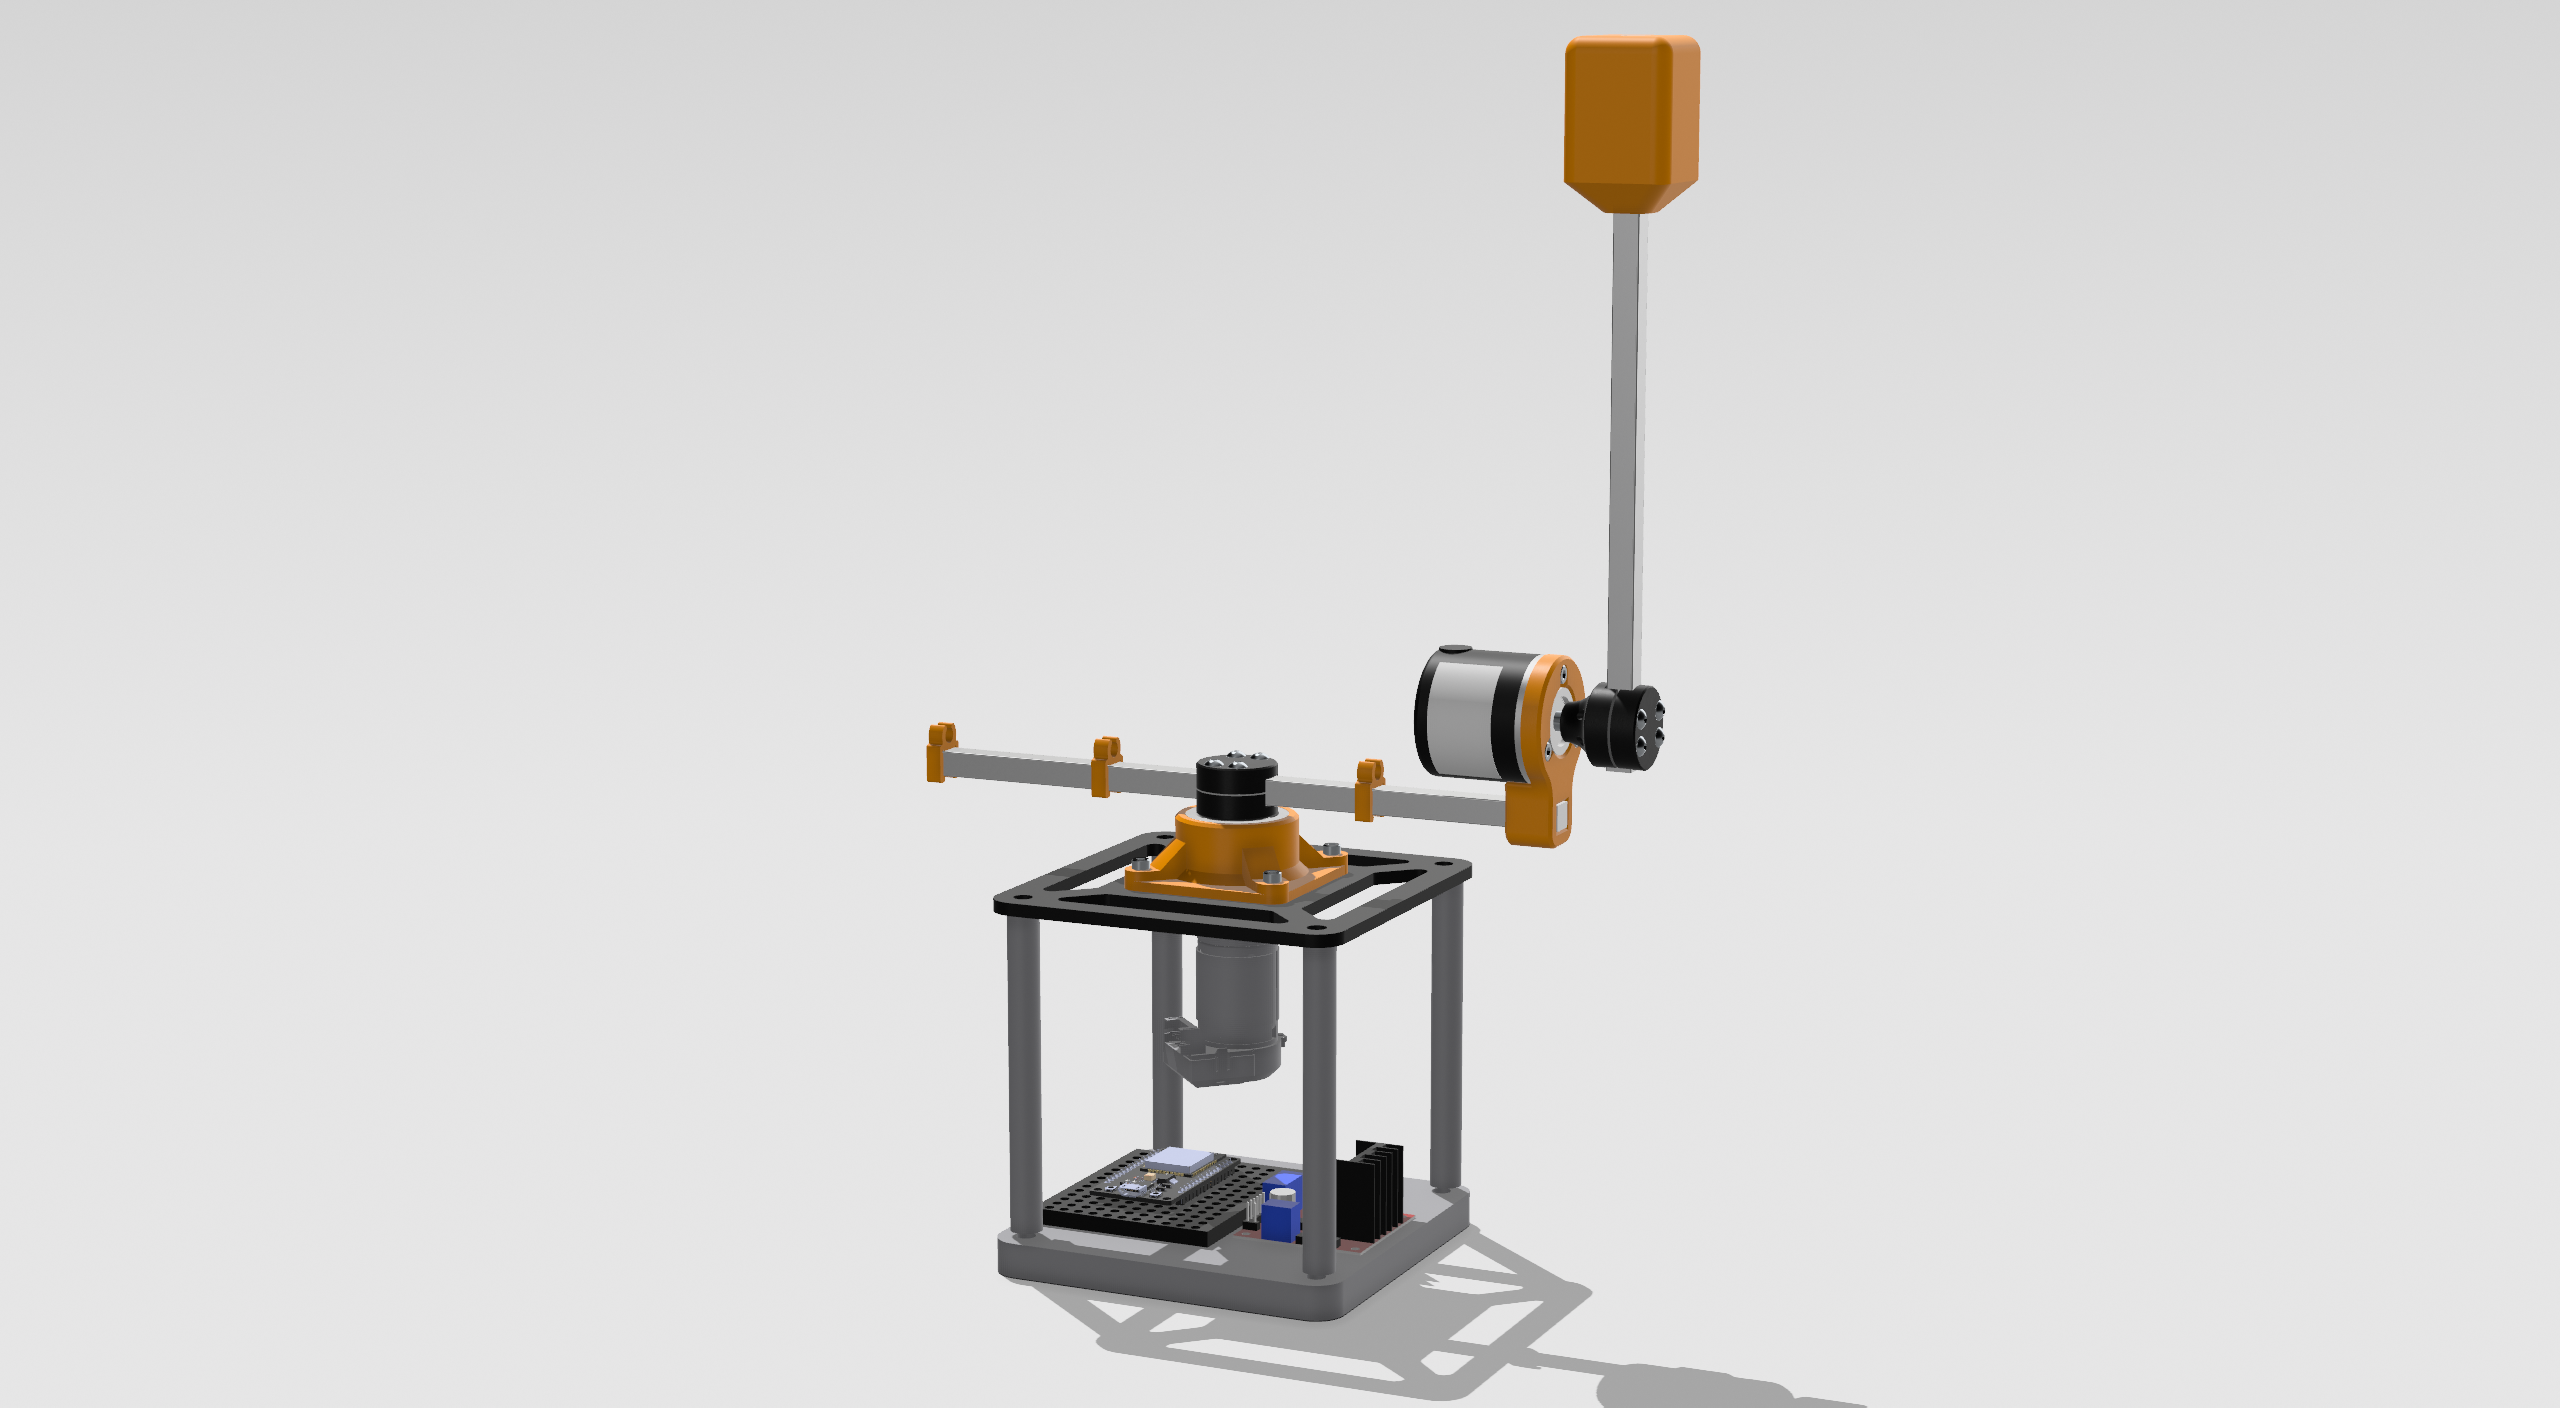
\includegraphics[width=0.7\textwidth]{res/metodologia/inv_pendulum.png}
  \caption{Pêndulo invertido rotativo}
  \label{fig:inv-pendulum}
\end{figure}

Perceba que a leitura dos sensores é realizada através de interrupção, enquanto o controle é realizado por uma tarefa. A interação entre os dois é imposta pela física da planta e necessita de sincronização por conta desta concorrência. Essa interação entre \ac{ISR} e Tarefa de controle se liga diretamente ao padrão P3 da taxonomia e esta interação é o padrão avaliado no experimento de custo (ver protocolo na seção \ref{sec:experiment-proc}). Note que a planta possui dois \textit{encoders}: um para o braço e outro para o pêndulo. Com isso, é necessário que essas duas informações sejam atualizadas em conjunto, pois caso uma seja atualizada e a outra ainda esteja com o valor antigo e estes valores sejam usados no controle, isso pode gerar um sinal de controle para corrigir um estado falso. Desta forma, é necessário que a atualização deste bloco coerente seja feita de forma única para evitar \textit{data races}.

Outro ponto importante a se destacar é a utilização do ESP32, com a arquitetura Xtensa, como microcontrolador. Com isso, este trabalho, por utilizar essa planta, fica restrito à utilização do ESP32 (Xtensa). Esse microcontrolador é representativo, pois é muito popular e barato. Apesar de este microcontrolador possuir dois núcleos, é utilizado apenas um dos núcleos. Isso já foi cortado na taxonomia, na subseção \ref{subsec:taxonomy}, na qual as células com o eixo Núcleo-Núcleo foram cortadas. Mesmo com esse corte, a corrida continua existindo entre a \ac{ISR} e a tarefa de controle, o que permite as medições dos custos neste caso, mesmo sendo \textit{single-core}.

Por fim, a execução é realizada em dois estágios: simulação e planta física. O objetivo é começar onde a implementação e os testes são mais fáceis, indo em direção a onde existe mais fidelidade. Observe que as medições são feitas na planta física e não na simulação. A simulação, neste caso, funciona como um ensaio, pois permite acelerar o desenvolvimento e depuração do controlador em um ambiente controlado.

% 4.6.2
\subsection{Implementações comparadas}

Nesta subseção, são especificadas as duas implementações que são usadas nos experimentos. A primeira é o estado da arte do que é utilizado para a implementação de controladores em sistemas embarcados e é usada como referência na medição dos experimentos, enquanto a segunda é a implementação que possui verificação de tipos e as garantias do lado \textit{safe} e é o alvo das medições dos experimentos. Além disso, essa subseção busca mostrar que essas duas abordagens são idênticas no que é controlável (com diferenças no substrato sendo tratadas na decomposição das medições), enquanto é variado o mecanismo que protege o bloco coerente do padrão P3 na fronteira \ac{ISR} e Tarefa. As escolhas da planta, do ESP32 \textit{single-core} e do padrão P3 são feitas na subseção \ref{subsec:plant-platform}, enquanto a escolha de FreeRTOS e \textit{bare-metal} é feita nesta subseção.

A primeira implementação é feita em cima da linguagem C, usando o FreeRTOS, provido no \ac{SDK} ESP-IDF e segue as linhas da especificação \ac{MISRA}. O FreeRTOS não foi uma escolha deliberada, mas o mais representativo quando se fala em desenvolver com ESP32, pois o \ac{SDK} deste microcontrolador, ao contrário de outros microcontroladores, não expõe um modo de execução em \textit{bare-metal}, mas sempre está em execução uma implementação do FreeRTOS. A especificação \ac{MISRA} traz dois fundamentos: o primeiro é forçar um C disciplinado ao invés de ingênuo. Isso faz com que a comparação com o Rust seja com o melhor código possível de C. Além disso, essa especificação também força o uso de memória estática (ou proíbe o uso de alocação dinâmica). Isso garante a simetria na alocação de memória com a segunda implementação em Rust, ao usar somente alocação estática. Como a \ac{ISR} escreve em um bloco coerente e a tarefa lê este bloco, a proteção contra leitura inconsistente deste bloco é feita através de seção crítica.

Na segunda implementação, onde o custo do Rust será medido, é usada a forma mais idiomática do Rust, para o ESP32 (Xtensa): Rust \textit{bare-metal} em \textit{no\_std}, com alocação estática usando o \textit{crate} heapless e utilizando o \textit{crate} esp-hal, como \ac{HAL}. Além disso, o compartilhamento entre \ac{ISR} e Tarefa será feito através de um bloco específico da biblioteca Aule, bem como todo o núcleo de controle \ref{subsec:catalog-n-unsafe-policy}. Perceba que o mais idiomático, neste caso, no Rust, não é utilizar um \ac{RTOS}, mas sim \textit{no\_std} \textit{bare-metal} com esp-hal. Isso ocorre, pois o \ac{RTIC} não suporta ESP32 Xtensa e o Embassy não é um \ac{RTOS} no mesmo sentido que o FreeRTOS, pois enquanto o FreeRTOS utiliza preempção no escalonamento, o Embassy utiliza cooperação no escalonamento. Com isso, o \textit{bare-metal} \textit{no\_std} com o esp-hal é a abordagem mais adequada e mais próxima que existe no Rust, para esse caso, com relação à implementação de referência. Para o regime de memória, é utilizado o \textit{crate} heapless, pois com ele é possível obter alocação estática e manter a simetria (no âmbito da garantia de P3) com a implementação de referência. Note que ainda é utilizada alocação dinâmica, mas não na garantia, apenas como escolha do veículo de instanciação Aule. O ponto diferente entre as duas implementações é que em \textit{safe} Rust, é impossível o compartilhamento de um bloco mutável sem um container de sincronização. O bloco coerente escrito na \ac{ISR} e lido pela Tarefa possui sua sincronização como opcional na implementação de referência, necessitando da disciplina do programador. Enquanto na implementação em Rust, por conta do sistema de tipos, a sincronização é forçada.

Na tabela \ref{tab:impl-compare} são mostradas as diferenças entre cada uma das implementações. A tabela é construída com quatro colunas: a primeira é a dimensão na qual é apresentado o item de cada implementação; a segunda coluna, a forma em que a primeira implementação (C+\allowbreak FreeRTOS+\allowbreak \ac{MISRA}) realiza o item; a terceira coluna, a forma em que a segunda implementação (Rust+Aule) realiza o item; e a última coluna, na qual é classificada a diferença entre a coluna 2 e 3 em um dos três grupos: Controlado, em que não há diferença; Variável de estudo, em que é feita a comparação das medições; e Variável de Confusão Neutralizada, em que existe uma diferença, mas é isolada por medição. Note que ambas as implementações protegem o bloco com a mesma primitiva: mascarar \ac{IRQ} com uma seção crítica. Isso indica que o que está sendo medido não é a primitiva em si, mas sim o custo que o container \textit{safe} do Rust adiciona sobre a primitiva compartilhada. O \textit{overhead} desse container ser desprezível indica a segurança sem custos adicionais.

\begin{table}[ht]
  \centering
  \caption{Comparação entre a implementação de referência e a implementação medida}
  \label{tab:impl-compare}
  \begin{tabularx}{\textwidth}{>{\hsize=0.5\hsize}X >{\hsize=1.0\hsize}X >{\hsize=1.5\hsize}X >{\hsize=1.0\hsize}X}
    \toprule
    Dimensão & C+\allowbreak FreeRTOS+\allowbreak MISRA & Rust+Aule & Papel no Experimento \\
    \midrule
    Algoritmo de controle & Realimentação de estados & Realimentação de estados & Controlado \\
    \hline
    Estimador & Kalman (mesma tarefa) & Kalman (planejado, mesma tarefa) & Controlado \\
    \hline
    Planta & Furuta física & Furuta física & Controlado \\
    \hline
    MCU & ESP32 Xtensa & ESP32 Xtensa & Controlado \\
    \hline
    Uso do núcleo & Single-core & Single-core & Controlado \\
    \hline
    Período e deadline & Escolhido pelo usuário & Escolhido pelo usuário & Controlado \\
    \hline
    Carga & Escolhida pelo usuário & Escolhida pelo usuário & Controlado \\
    \hline
    Caso & P3 (fronteira ISR-Tarefa) & P3 (fronteira ISR-Tarefa) & Controlado \\
    \hline
    Aquisição de dados & Interrupção & Interrupção & Controlado \\
    \hline
    Memória da garantia & heap-free & heap-free & Controlado \\
    \hline
    Mecanismo de proteção do bloco & Mascarar IRQ (seção crítica) & Mascarar IRQ (seção crítica) & Controlado \\
    \hline
    Acesso do mecanismo de proteção & Direto (sob seção crítica) & \texttt{Mutex<RefCell>} & Variável de estudo \\
    \hline
    Substrato & Free-RTOS & bare-metal & Variável de Confusão Neutralizada \\
    \hline
    Alocação de veículo & 100 \% estática por MISRA & Heap no observador & Variável de Confusão Neutralizada \\
    \bottomrule
  \end{tabularx}
\end{table}

Por fim, a tabela mostra que as dimensões estão controladas ou a variável de confusão foi neutralizada, só restando a diferença na variável de estudo, a qual queremos medir. Esta variável indica o quanto a adição de segurança do Rust custa. Se esse custo for desprezível, ou seja, um empate entre as duas implementações, então o Rust possui uma segurança sem custos. Entretanto, caso não exista o empate, o custo do lado \textit{safe} do Rust fica quantificado.

% 4.6.3
\subsection{Métricas e instrumentação}

Na subseção \ref{subsec:cost-impl} são apresentadas quatro dimensões qualitativas: \textit{Runtime}, Determinismo, \textit{Footprint} e Ergonomia, enquanto isso, nesta subseção é apresentado o protocolo de medição para cada dimensão. Além disso, também é apresentada a decomposição que mostra como a neutralização de cada uma das variáveis de confusão é realizada.

O protocolo de medição consiste em estabelecer quatro propriedades para cada dimensão: a grandeza, indicando o que será medido; como medir esta grandeza; a unidade desta grandeza; e quando será feita a medição: estático (no build) ou em \textit{runtime} (na planta). Note que aqui é definido somente o protocolo, nenhuma medição é feita.

Para a dimensão de \textit{Runtime}, é utilizado como grandeza a quantidade de ciclos de \ac{CPU} na região de interação do bloco coerente. A unidade é ciclos e não tempo, pois com ciclos tem-se independência do clock. A medição desta grandeza é feita através de um delta do valor do registrador CCOUNT, em que a medição é feita ao redor da região de acesso ao bloco coerente. Deve ser anotado o delta da região com o bloqueio e o código e da mesma região com o bloqueio mas vazia. A medição com a região vazia é usada como referência para a comparação. A medição é feita em \textit{runtime} (na planta).

Já na dimensão de Determinismo, tem-se três sub-métricas: \textit{Jitter}, \textit{Deadline} perdido e Inversão de prioridade. São utilizadas três sub-métricas, pois cada uma mostra uma informação importante: \textit{jitter} mostra a variabilidade, \textit{deadline} perdido mostra a falha crítica e a inversão de prioridade mostra o custo imposto ao outro contexto. Todas as sub-métricas são medidas em \textit{runtime} (na planta). A primeira sub-métrica é o \textit{jitter}. Nele é medida a dispersão da distribuição de ciclos sobre N iterações. Para calcular o \textit{jitter}, é necessário escolher uma estatística. As estatísticas mais comuns são: desvio-padrão, p99-mediana e amplitude máximo-mínimo.

A primeira estatística é o desvio-padrão. Essa estatística é mais complexa de ser calculada, mas possui maior resistência a outliers. Entretanto, ainda possui um problema com distribuições com caudas pesadas e assimétricas, o que é o caso de latências em sistemas reais. O problema do desvio padrão é subestimar a cauda e permanecer pequeno, mesmo com iterações raras ruins. A segunda estatística é o p99-mediana, em que a mediana é o valor central da distribuição e o p99 é o valor em que 99\% dos valores caem abaixo. Com a diferença desses valores é possível medir o tamanho da cauda superior, acima do valor típico. Na amplitude máximo-mínimo é calculada a diferença entre o valor máximo e mínimo observado. Essa estatística é fácil de ser calculada, porém é muito sensível a valores máximos, por isso é a estatística utilizada. Para eliminar possíveis outliers é avaliada a distribuição para validar se o valor máximo é um ruído ou não. A unidade utilizada é novamente ciclos. O \textit{deadline} perdido é medido pela quantidade de \textit{deadlines} perdidos por cada execução. Para marcar um \textit{deadline} como perdido, o tempo de resposta do sinal de controle deve ser maior do que o período de controle, que é de 2\,ms para essa planta. Esse valor foi obtido empiricamente pelo fabricante da planta e está descrito no firmware original da planta \citep{furuta-plant}. Além disso, esse período pode ser convertido para ciclos usando o clock da \ac{MCU}, que permanece fixo durante todas as medidas. E a última métrica é a inversão de prioridade. Aqui, é mascarada a \ac{IRQ} através de uma seção crítica e com ela mascarada o contexto de mais alta prioridade é impedido de executar até a seção crítica acabar. Com isso, é medido o atraso, em ciclos, em que a \ac{ISR} deveria começar a executar até ela de fato executar.

Na dimensão três tem-se o \textit{footprint} de memória. Nela são medidos os bytes usados na \ac{RAM} (nas seções .data e .bss) e na Flash (na seção .text). Essa medida é feita em cada uma das implementações: de referência e de medição. A medição é estática, feita no build com o binário de cada implementação. Note que a medição deve ser da adição da garantia. Desta forma, é medido com e sem a garantia para saber quantos bytes foram adicionados por conta da garantia. Na versão Rust, por não ser possível compilar sem a garantia, é compilado com a região de bloqueio vazia e sem a região de bloqueio. Com isso, é possível ter a diferença entre os dois casos e isolar somente a adição das garantias. Para evitar a otimização do compilador da região vazia são adicionadas barreiras de otimização nesta região.

E por último, a dimensão de ergonomia. Nela é medida a quantidade de \textit{boilerplate} adicionado pelas garantias. A unidade de medida é Linhas de Código (\ac{LoC}). Para o \textit{boilerplate} são consideradas as linhas de interação com \textit{mutexes} e atômicos. O momento de medição é estático, pois só necessita da quantidade de linhas escritas.

Algumas ressalvas devem ser feitas aqui sobre a influência do custo da leitura do CCOUNT. O primeiro é sobre a influência da leitura do CCOUNT na variável de estudo. O custo de leitura entra como aditivo em cada delta de leitura. Como na variável de estudo é realizada uma diferença entre duas medições (um delta), o custo de leitura é eliminado porque é feita uma diferença desse delta (delta de medição com código versus delta de medição com região vazia). O segundo local onde o custo de leitura influencia é no \textit{jitter}. Lá não são feitas diferenças pareadas, mas como a variância desse custo de leitura é desprezível (a verificar nos experimentos), então esta não terá influência no resultado do \textit{jitter}. O último ponto é onde são calculados valores absolutos, como \textit{deadline} e inversão de prioridade. Nesse ponto, não existe influência pois a diferença de magnitude é muito grande, já que o custo da leitura é poucos ciclos, enquanto esses valores estão na ordem de centenas de milhares de ciclos (milissegundos). Outro ponto para se notar sobre as medições é que são obtidos valores sobre várias iterações e não em uma simples medição. Desta forma, obtemos uma distribuição, na qual a validação dos valores obtidos é muito mais confiável do que uma simples medição, a qual é passível de aleatoriedade. Note que aqui foi discutido como é eliminado o custo da leitura e não o custo do FreeRTOS.

Neste momento é tratado o custo do FreeRTOS. Isso é importante, pois existe uma assimetria entre as duas implementações: na implementação C+FreeRTOS existe um custo do tick do FreeRTOS, enquanto no Rust+baremetal, isso não existe. Note que os ticks do FreeRTOS ocorrem fora da região de medição, pois dentro da região a \ac{IRQ} está mascarada. Desta forma, a variável de estudo não é afetada, apenas o \textit{deadline} e a inversão de prioridade. Para explicitar essa adição de custo, será medida a quantidade de ciclos por tick do FreeRTOS e esse valor será multiplicado pela frequência de ticks do FreeRTOS. Com esse resultado, esse valor é explicitado para mostrar o quanto o valor de \textit{deadline} foi afetado. Note também que o \textit{jitter} não é afetado pelos ticks do FreeRTOS, pois ele é medido na janela com a seção crítica. Um outro ponto é o uso de \textit{heap}, o qual é assimétrico entre as implementações. O bloco do observador Kalman possui alocação dinâmica no Rust, enquanto em C não existe. Entretanto, essa alocação é realizada previamente e não na janela de medição. Além disso, a alocação dinâmica é um custo do veículo, e não da garantia. Note que a garantia permanece \textit{heap-free} nas duas implementações.

Com esses pontos observados, é possível notar que apenas a variável de estudo possui diferenças não atribuídas às variáveis de confusão. Os desfechos possíveis entre as duas implementações são: um empate, em que o delta entre elas é desprezível, indicando que o Rust possui, neste caso, uma \textit{zero-cost} abstraction; e um não-empate, em que o custo do lado \textit{safe} do Rust é quantificado. Nesta subseção foi descrito o que medir e como medir, na subseção \ref{subsec:quantity-measurement} é descrito (ou adiado) o quanto de cada medida.

% 4.6.4
\subsection{Limites entre qualificação e dissertação}
\label{subsec:quantity-measurement}

Note que esta seção (\ref{sec:experiment-proc}) define que a fase de qualificação entrega apenas o projeto do que será medido no experimento de custo, ou seja, o que e como será medido. A medição em si, fica na fase da dissertação. Esta seção busca a hipótese testável e isso foi alcançado definindo: o critério qualitativo central, em que o \textit{data race} cai do lado \textit{safe} e não compila, sendo forçado à forma segura; os quatro eixos quantitativos operacionalizados, sendo eles definidos por: grandeza, como é medido, a unidade e quando ocorre a medição; a validade interna de cada medição, mostrando o que é controlado entre as duas implementações, as variáveis de confusão entre as implementações e como elas são decompostas e resolvidas e o que sobra é somente a variável de estudo. E por fim, a hipótese de que se a medição for empate é custo zero para o Rust e se não houver empate é medido o custo da garantia do Rust.

Desta forma, o que é adiado para a dissertação é o quanto de cada medida. Essas definições adiadas são: os thresholds numéricos, por exemplo: qual o threshold deve ser ultrapassado para as medidas não serem consideradas um empate. O valor é adiado, mas como ele é obtido é definido da seguinte forma: a diferença entre o máximo e o mínimo do ruído medido na região vazia; a escala das medições, isto é: o número de repetições para coletar as distribuições. Da mesma forma que a definição anterior, o valor é adiado, mas como é medido é definido agora: a quantidade em que a distribuição estabiliza, ou seja, para de mudar; a variante específica da ESP32 utilizada na planta física; e, por fim, a execução desses valores na planta física. Note que todas essas definições dependem da execução e testes na planta física. Fazer essas definições sem valores reais seria arbitrar valores podendo ter um descasamento com condições reais observadas no momento do experimento. Portanto, como esse trabalho segue o sequenciamento exploratório $\rightarrow$ empírico, a parte empírica fica adiada para a dissertação.

% 4.7
\section{Verificação por Tipos vs. C+MISRA+\textit{Sanitizers}}
\label{sec:type-system-vs-sanitizer}

% 4.7.1
\subsection{Dimensão de comparação}
\label{subsec:dim-comp}

Nesta seção é tratada a comparação entre o regime de verificação de erro em \textit{data races} de cada implementação. Por um lado, tem-se o Rust \textit{safe}, com o sistema de tipos e, por outro lado, o C+\ac{MISRA}+\textit{Sanitizers}, com disciplina mais ferramentas de verificação em \textit{runtime}. Note que a abordagem do C+\ac{MISRA}+\textit{Sanitizers} não é uma abordagem ingênua, mas o estado da arte da implementação segura em C. Para que a comparação dessas duas abordagens seja justa é necessário que as regras valham para ambos os lados. Desta forma, para ambos os lados serão usados os mesmos padrões de \textit{data race} (desde o P1 até o P4 da taxonomia), pois com isso tanto o C quanto o Rust enfrentam o mesmo padrão. Também é utilizado o mesmo alvo, pois é onde mora o problema, por exemplo no caso em que uma \ac{ISR} e uma Tarefa disputam o mesmo recurso. E por último o mesmo algoritmo de controle, pois em ambos os casos é comparada a realimentação de estados do pêndulo. Portanto, o que varia é o regime de verificação de erros.

Sendo assim, será descrita aqui uma lista de dimensões. Cada dimensão é uma pergunta feita para cada um dos lados e são obtidas duas respostas, uma para cada lado. Primeiramente, temos o momento da verificação, em que se quer saber quando o problema é pego. Em C, é em tempo de execução, já em Rust é em tempo de compilação. Também tem-se a natureza da garantia, em que se pergunta o que ocorre com o \textit{bug}. Em C, o problema é detectado em um caso em execução, já em Rust o problema é prevenido por construção. Após isso, é perguntado qual o esforço para localizar os \textit{bugs}. Em C, deve-se utilizar ferramentas externas e revisão humana, enquanto em Rust o sistema de tipos previne esses \textit{bugs}. E a última pergunta é: onde é delimitado o código inseguro. Em C, pode ser qualquer parte do código, enquanto em Rust, é delimitado pelas linhas de código marcadas pelo bloco \textit{unsafe}.

Note que a pergunta central é o momento onde o problema é tratado, pois em C são procurados problemas que ocorrem em tempo de execução. Isso é problemático, pois é necessário esperar o problema ocorrer e esse problema pode estar escondido e nem ocorrer no momento do desenvolvimento, apenas sendo mostrado em produção. O que é diferente do Rust, em que os problemas são prevenidos em compilação. Isso significa que esse problema nunca será apresentado em produção, pois ele nem sequer é executado, pois não compila.

Nas seções seguintes será tratada a instanciação de cada dimensão \ref{subsec:dim-inst}, bem como quais são os limites que essas dimensões atingem \ref{subsec:dim-bounds}.

% 4.7.2
\subsection{O artefato comparativo}
\label{subsec:dim-inst}

Note que na subseção \ref{subsec:dim-comp} foram declaradas dimensões para a comparação qualitativa entre as abordagens, aqui é mostrado como serão construídos os três elementos para a comparação e onde mora cada dimensão. Nesta subseção é construído o protocolo de construção do trio, o trio preenchido fica para a seção de resultados. Os três elementos são: um snippet em C (com \ac{MISRA}), que compila e roda com o \textit{bug} latente (elemento 1). Neste caso o \textit{bug} está latente e pode ou não se manifestar em tempo de execução; o mesmo padrão em Rust \textit{safe} que não compila, por conta do sistema de tipos (elemento 2); e o diagnóstico do \textit{sanitizer} sobre o C implementado (com \ac{MISRA}), caso o caminho que contém o \textit{bug} seja executado (elemento 3). Note que é realizado um trio por padrão do P1 até o P4, da taxonomia.

Perceba que é necessário ter um trio (com o terceiro elemento) pois a comparação do Rust \textit{safe} com o C ingênuo é injusta. Desta forma, é comparado com o C com \textit{sanitizer} e com \ac{MISRA}, para ter o C na sua melhor forma. A adição do \ac{MISRA} torna o C disciplinado, mas não automatiza a eliminação de \textit{data race}, pois é uma convenção em conjunto com uma análise estática incompleta. Deste modo, ainda é necessário o \textit{sanitizer} para pegar os \textit{bugs} em \textit{runtime}. O elemento 1 e o elemento 3 são o mesmo código, o que muda é que no elemento 3 existe a instrumentação por meio do \textit{sanitizer}. Outro ponto a se destacar é que o \textit{sanitizer} roda no estágio de simulação no host. Isso não tira o mérito da comparação, visto que o intuito é detectar o \textit{bug} de \textit{data race} que ocorre mesmo no host, não sendo dependente da ESP32 Xtensa. Outra diferença são os contextos nos quais serão executados, na ESP32 Xtensa é a interação entre \ac{ISR} e Tarefa, enquanto no host é Tarefa com Tarefa. Isso não os torna incompatíveis, uma vez que tanto \ac{ISR} e Tarefa, quanto Tarefa e Tarefa, (neste caso) caem no mesmo padrão da taxonomia.

Além disso, o trio satisfaz cada uma das dimensões descritas em \ref{subsec:dim-comp} da seguinte forma: a dimensão momento no elemento 2 é em tempo de compilação, enquanto no elemento 3 é em tempo de execução. Já no elemento 1, esse \textit{bug} não é detectado só aparecendo em produção. Sobre a natureza, tem-se que o elemento 2 previne pois não compila, enquanto o elemento 3 detecta num caso específico observado. O esforço do elemento 1 e 3 exige ferramenta extra, execução, além da revisão humana, enquanto no elemento 2 o próprio compilador acusa o problema. E a fronteira insegura, no elemento 2, é demarcada por blocos \textit{unsafe}, enquanto nos elementos 1 e 3 é todo o código C.

Para que se possa obter os mesmos resultados basta compilar o código, em Rust, e rodar o \textit{sanitizer} em C. Note que a compilação em Rust é determinística e sempre vai produzir o mesmo resultado, enquanto a detecção via \textit{sanitizer} depende do caminho do \textit{bug} ser exercitado durante a execução. Além disso, perceba que existem \textit{bugs} que o \textit{sanitizer} não consegue detectar e isso favorece a implementação em \textit{safe} Rust, pois C, na sua melhor forma, ainda tem limites em que não é possível detectar \textit{bugs}. Esses limites serão tratados na subseção \ref{subsec:dim-bounds}.

% 4.7.3
\subsection{Limites do \textit{sanitizer}}
\label{subsec:dim-bounds}

Visto que a subseção \ref{subsec:dim-inst} indica limites no \textit{sanitizer} em C, é necessário não só descrever estes limites nesta subseção, mas também os limites do próprio Rust \textit{safe}. Começando pelo \textit{sanitizer}, o primeiro limite a se destacar é a cobertura dinâmica realizada pelo \textit{sanitizer}. O \textit{sanitizer} só consegue observar o programa em execução. Com isso, ele só consegue detectar o \textit{bug} que é exercitado pelo programa que está executando. Se o \textit{bug} não for executado, ele vai passar despercebido pelo \textit{sanitizer}. Isso gera um não determinismo na saída do \textit{sanitizer}. A ausência de \textit{bugs} capturados pelo \textit{sanitizer} não significa que o código não possui \textit{bugs}, apenas que eles não foram exercitados. Além disso, o \textit{sanitizer} \ac{TSan} é específico para \textit{data races}, não sendo capaz de detectar problemas de memória como \textit{use-after-free} e \textit{lifetime}. O \textit{sanitizer} \ac{ASan} é capaz de detectar esses \textit{bugs}, enquanto o \textit{sanitizer} \ac{UBSan} detecta Undefined-Behaviors. Note que para pegar todos esses \textit{bugs} foram necessários três \textit{sanitizers} e três execuções separadas, pois cada \textit{sanitizer} exige uma compilação e execução separada, enquanto somente o compilador de Rust é capaz de lidar com todos eles. Esses \textit{bugs} não são o foco deste trabalho, mas são importantes para mostrar o limite de cada \textit{sanitizer} utilizado em C e que cada um deles não resolve todos os problemas.

Agora, note que o Rust \textit{safe} também possui seus limites. Apesar de prevenir \textit{data races}, ele não previne \textit{race conditions} lógicas, como: \textit{deadlocks}, ordem de operações e inversão de prioridade. Também não elimina o \textit{unsafe} na borda de hardware. Isso significa que compilar é não ter \textit{data race} exprimível, o que não quer dizer que o programa está logicamente correto.

Note que este trabalho afirma que no Rust existe um ganho na prevenção de \textit{data races}, por deslocar a verificação para a compilação determinística, ao invés de verificações não-determinísticas em \textit{runtime}. Essa afirmação não cobre todos os \textit{bugs} de memória, pois o intuito aqui é ser representativo e não exaustivo. Além disso, o \textit{unsafe}, apesar de continuar existindo no Rust, é pequeno, isolado e auditável.

Por fim, nesta seção foi apresentada a diferença entre a verificação por tipos e o estado da arte do C (com \ac{MISRA} e \textit{sanitizers}). Na subseção \ref{subsec:dim-comp} são apresentadas as dimensões para a comparação, na subseção \ref{subsec:dim-inst} é apresentado o trio que instancia as dimensões e na subseção \ref{subsec:dim-bounds} os limites do elemento 2 e 3 do trio de comparação. Nesta seção o foco foi mostrar a construção do protocolo de comparação, enquanto os resultados desta comparação serão mostrados no capítulo de resultados.

Neste capítulo, na seção \ref{sec:research-kind} é descrita a caracterização deste trabalho. Já na seção \ref{sec:taxonomy} é apresentada uma taxonomia com padrões de \textit{data races}. Na seção \ref{sec:border} é apresentada a fronteira entre o \textit{safe} e \textit{unsafe} nos padrões de \textit{data race}. Enquanto nas seções \ref{sec:cost} e \ref{sec:experiment-proc} são descritos os custos dos padrões encontrados. Além disso, na seção \ref{sec:aule} é descrito o meio que instancia cada um dos padrões. E por último na seção \ref{sec:type-system-vs-sanitizer} é descrito o regime de verificação de cada implementação.

     \mychapter{Resultados Parciais}{cap:Resultados Parciais}
\label{cap:experiment}

% 5.1
\section{Estado atual da biblioteca Aule}
\label{sec:aule-state}

% 5.2
\section{Caso demonstrativo: setpoint escalar compartilhado (P1)}
\label{sec:case-setpoint}

% 5.2.1
\subsection{Cenário e o padrão P1}
\label{subsec:setpoint-scenario}

Nesta seção será apresentado um caso de compartilhamento de um escalar entre duas tarefas. Esse dado compartilhado é uma referência, cujo controlador deve perseguir, através do envio de um sinal de controle. Com isso, uma tarefa escreve neste valor compartilhado, enquanto a outra, lê este valor. A tarefa responsável por ler o valor é a tarefa de controle, onde o controlador está atuando e precisa desse valor de referência em intervalos fixos de tempo, para conseguir seguir a referência. A tarefa que escreve o valor é uma tarefa de interação com o meio externo (ou com o usuário). Desta forma, esta tarefa recebe um valor de forma assíncrona e precisa escrever esse valor na variável de referência (ou setpoint). Essa forma de interação é comum, pois o usuário pode, por exemplo, alterar o valor de referência em uma IHM, e esse valor é recebido pela tarefa sem aviso ou intervalo definido. É recebido no momento em que o usuário decide alterar. Essa interação pode gerar uma leitura de valor obsoleto na tarefa de controle, pois o acesso ao valor não é indivisível e ordenado.

Note que neste caso, existem: 2 tarefas; um valor compartilhado escalar, por exemplo, a altura de um tanque, ou a velocidade de um motor, ou a temperatura de uma câmara, etc.; e uma tarefa que se comporta como leitora e outra que se comporta como escritora. Esse caso é mapeado exatamente para o caso P1 da taxonomia (\ref{subsec:taxonomy}), onde o trio é composto por $\langle \text{Tarefa-Tarefa},\text{Escalar},\text{Leitor-Escritor}\rangle$. Note que a referência é um valor escalar, logo ela cabe em uma operação atômica. Isso corta o caso P3. Além disso, o valor atual não depende do valor anterior, o que corta o caso P4.

Visto que a biblioteca Aule é o veículo onde o loop de controle vive, é esperado que ela seja utilizada neste exemplo. Entretanto, ela não será utilizada por 2 motivos que se complementam: o primeiro é que o P1 mora na borda entre a tarefa de comunicação e a tarefa de controle e não no núcleo de controle. Com isso, utilizar Aule, neste caso, não traria ganhos para analisar o caso P1 proposto. Consequentemente, o segundo motivo vem deste, pois usar Aule poderia passar a ideia que a garantia mostrada vem da biblioteca e não da linguagem Rust. Para casos onde realmente existe um algoritmo de controle em execução, como, por exemplo, na planta de controle física, o uso da biblioteca Aule é essencial. Na próxima subseção (\ref{subsec:setpoint-c}) é mostrado o código em C que instancia o caso descrito na subseção atual.

% 5.2.2
\subsection{O data race em C}
\label{subsec:setpoint-c}

Na listagem \ref{code:data-race-c}, é apresentado o trecho de código em C, que possui o data race apresentado em \ref{subsec:setpoint-scenario}. Neste código a variável \texttt{g\_setpoint} é compartilhada entre a tarefa \texttt{comm\_task} (escritora) e a tarefa \texttt{control\_loop} (leitora). Note que a variável \texttt{g\_setpoint} não possui nenhuma sincronização.

\codec{Data race (P1) de setpoint compartilhado entre leitor-escritor}{code:data-race-c}{src/p1/setpoint.c}

Para que o trecho apresentado seja um data race, ele deve atender a definição de data race, descrita em \ref{sec:dr-def}. Nela, um data race deve possuir: 2 contextos, cumprido com a tarefa leitora e a tarefa escritora; pelo menos 1 escrita, cumprido com a tarefa escritora; acesso não-atômico, cumprido, pois o acesso é direto; e sem happens before, cumprido, pois com o acesso direto não existem restrições para o compilador (ou processador) reordenar as instruções de acesso. Com as quatro condições atendidas, o trecho de código em C configura-se como um data race e note que é o lado indivisível e ordenado do acesso que falha.

Mesmo com o data race presente, o compilador compila sem erro ou aviso e permite que o programa seja executado sem falha aparente. Ou seja, o programa é executado com um bug latente, onde a leitura do valor do controlador pode ser inconsistente e gerando um sinal de controle errado e uma saída não-determinística. Note que esta é a versão ingênua do C, justamente porque esse é o jeito natural de escrever em C e o compilador não impede o desenvolvedor de escrever assim. Para encontrar este data race, é possível executar o sanitizer TSan e confirmar. Na listagem \ref{code:tsan-out}, é possível ver a saída do TSan informando a presença de data race na variável \texttt{g\_setpoint}.

\begin{lstlisting}[
    caption={Saída do TSan no caso P1 (na linguagem C)},
    label={code:tsan-out},
    basicstyle=\footnotesize\ttfamily,
    breaklines=true,
    frame=shadowbox, rulesepcolor=\color{gray}]
==================
WARNING: ThreadSanitizer: data race (pid=5128)
  Write of size 4 at 0x000100fb8000 by thread T1:
    #0 comm_task setpoint.c:18 (setpoint-tsan:arm64+0x100000824)

  Previous read of size 4 at 0x000100fb8000 by thread T2:
    #0 control_loop setpoint.c:32 (setpoint-tsan:arm64+0x1000008c4)

  Location is global 'g_setpoint' at 0x000100fb8000 (setpoint-tsan+0x100008000)

  Thread T1 (tid=5084491, running) created by main thread at:
    #0 pthread_create <null> (libclang_rt.tsan_osx_dynamic.dylib:arm64e+0x33834)
    #1 main setpoint.c:49 (setpoint-tsan:arm64+0x100000718)

  Thread T2 (tid=5084492, running) created by main thread at:
    #0 pthread_create <null> (libclang_rt.tsan_osx_dynamic.dylib:arm64e+0x33834)
    #1 main setpoint.c:50 (setpoint-tsan:arm64+0x100000730)

SUMMARY: ThreadSanitizer: data race setpoint.c:18 in comm_task
==================
\end{lstlisting}

Perceba que apesar do TSan encontrar este caso, foi necessário executar o programa e exercitar o bug. Em fluxos mais complexos o TSan pode não capturar o data race, por este ainda não ter sido exercitado. Uma recusa determinística e em tempo de compilação, facilitaria a prevenção deste data race com mais segurança.

% 5.2.3
\subsection{A recusa do compilador em Rust safe}
\label{subsec:setpoint-reject}

Recusar determinísticamente e em tempo de compilação é justamente o que a linguagem Rust faz. Aqui é usado o mesmo cenário da subseção anterior (\ref{subsec:setpoint-c}), instanciando o caso P1: duas tarefas compartilhando um valor, sem sincronização, onde uma é leitora e a outra escritora. É importante salientar que para um valor static ser compartilhado entre duas tarefas, em Rust, é necessário que esse valor seja \texttt{Sync}.

Na listagem \ref{code:setpoint-safe} é apresentado o trecho de código em Rust para este cenário. Esse trecho de código é uma implementação ingenua, onde é implementado uma transposição direta do código implementado em C. Neste código, temos o valor compartilhado na linha 6: um static com o tipo \texttt{Cell<f32>}, esse valor permite uma mutabilidade interior natual, já que em Rust safe não é permitido acessar uma variável mutável e static (que dure todo o lifetime do programa). Para acessar isso é necessário usar blocos unsafe. Da mesma forma que o cenário em C, existem duas tarefas: uma para ler setpoints do usuário, por meio do stdin. Esta é a tarefa escritora, pois recebe o valor do usuário e escreve na variável compartilhada; e a outra tarefa é o loop de controle, a qual lê o valor da variável compartilhada (setpoint) a cada ciclo do controle (tarefa leitora).

\coderust{Data race (P1) de setpoint compartilhado entre leitor-escritor, em Rust safe}{code:setpoint-safe}{src/p1/setpoint_safe.rs}

\begin{lstlisting}[
    caption={Saída do compilador rustc, sobre a implementação ingenua de Rust no caso P1},
    label={code:rustc-error},
    basicstyle=\footnotesize\ttfamily,
    breaklines=true,
    frame=shadowbox, rulesepcolor=\color{gray}]
\end{lstlisting}

Ao compilar o trecho de código \ref{code:setpoint-safe}, é apresentado um erro de compilação, descrito na listagem \ref{code:rustc-error}. Neste erro de compilação é apresentado o motivo da falha da compilação: o tipo \texttt{Cell<T>} não implementa a trait \texttt{Sync}, logo a variável de setpoint (na linha 6) não pode ser compartilhada entre as tarefas. Isso mostra a recusa do compilador sobre o data race presente no código \ref{code:setpoint-safe}. Note que, o valor possuir 2 acessos concorrentes e sem sincronização fica inexpremível na linguagem Rust, pois o código nem compila. O que é diferente de C, que permite a compilação e execução do código com data race. Perceba também que o problema foi pego em tempo de compilação e não foi necessário exercitar o código, como acontece na detecção em C, com o sanitizer TSan. Isso fornece justamente o que a subseção \ref{subsec:setpoint-c} buscava: uma forma de detectar o problema em tempo de compilação e de forma deterministica, uma vez que não depende de exercitar o código e o resultado do compilador é sempre o mesmo para a mesma entrada (o mesmo código).

Apesar de mostrar de forma deterministica e em tempo de compilação o problema, ainda não é apresentado a forma de remover o data race. Na próxima subseção \ref{subsec:setpoint-atomic}, é apresentado como resolver isso em Rust.

% 5.2.4
\subsection{A forma segura com atomic}
\label{subsec:setpoint-atomic}

% 5.2.5
\subsection{Leitura do caso como evidência}
\label{subsec:setpoint-evidence}

% 5.3
\section{Limitações conhecidas}
\label{sec:partial-limitations}

     \mychapter{Cronograma de Execução}{cap:Cronograma de Execução}
\label{cap:cron}

\section{Calendário}

\section{Plano de Trabalho}

    \include{capitulos/conclusao}
\appendix
% modified-by: Claude (claude-opus-4-8), 2026-08-07 -- titulo manual esvaziado (a designacao
% "Apendice A" ja e automatica apos \appendix); reguas por linha e 1a coluna alargada.
% Autorizado por Matheus (suspensao pontual da Regra 3).
\chapter[Apêndice A]{}
\label{cap:apendix-a}

% added-by: Claude (claude-opus-4-8), 2026-07-28 -- transposicao de res/pids.csv (dado levantado por Matheus) via csvsimple; autorizada por ele nesta data
\begin{landscape}
  \scriptsize
  \setlength{\tabcolsep}{2pt}
  % pdflscape mantem a \textwidth do retrato; reatribui para a dimensao que vira horizontal apos girar
  \setlength{\textwidth}{\textheight}%
  \setlength{\linewidth}{\textwidth}%
  \begin{longtable}{>{\raggedright\arraybackslash}p{4cm} *{18}{c} >{\raggedright\arraybackslash\scriptsize}p{4.2cm}}
    \caption{Levantamento dos repositórios de PID em Rust (lista congelada em 09/06/2025)}
    \label{tab:pid-survey} \\
    \toprule
    \textbf{Name}
      & \rotatebox{90}{embedded setpoint~}
      & \rotatebox{90}{mutable setpoint~}
      & \rotatebox{90}{mutable kp,ki,kd~}
      & \rotatebox{90}{generic typing~}
      & \rotatebox{90}{anti-windup~}
      & \rotatebox{90}{output-limit~}
      & \rotatebox{90}{Deadband~}
      & \rotatebox{90}{no\_std~}
      & \rotatebox{90}{library/binary~}
      & \rotatebox{90}{Documentation~}
      & \rotatebox{90}{Statistics~}
      & \rotatebox{90}{CI~}
      & \rotatebox{90}{crates.io~}
      & \rotatebox{90}{tests~}
      & \rotatebox{90}{Plot~}
      & \rotatebox{90}{benches~}
      & \rotatebox{90}{Examples~}
      & \rotatebox{90}{RK4 Integrator~} & \textbf{URL} \\
    \midrule
    \endfirsthead
    \multicolumn{20}{c}{\tablename\ \thetable{} -- continuação} \\
    \toprule
    \textbf{Name}
      & \rotatebox{90}{embedded setpoint~}
      & \rotatebox{90}{mutable setpoint~}
      & \rotatebox{90}{mutable kp,ki,kd~}
      & \rotatebox{90}{generic typing~}
      & \rotatebox{90}{anti-windup~}
      & \rotatebox{90}{output-limit~}
      & \rotatebox{90}{Deadband~}
      & \rotatebox{90}{no\_std~}
      & \rotatebox{90}{library/binary~}
      & \rotatebox{90}{Documentation~}
      & \rotatebox{90}{Statistics~}
      & \rotatebox{90}{CI~}
      & \rotatebox{90}{crates.io~}
      & \rotatebox{90}{tests~}
      & \rotatebox{90}{Plot~}
      & \rotatebox{90}{benches~}
      & \rotatebox{90}{Examples~}
      & \rotatebox{90}{RK4 Integrator~} & \textbf{URL} \\
    \midrule
    \endhead
    \midrule
    \multicolumn{20}{r}{continua na proxima pagina} \\
    \endfoot
    \bottomrule
    \endlastfoot
    \csvreader[respect underscore, no check column count, separator=comma, late after line=\\\hline]%
      {res/pids.csv}{}{%
      \csvcoli & \csvcolii & \csvcoliii & \csvcoliv & \csvcolv & \csvcolvi
      & \csvcolvii & \csvcolviii & \csvcolix & \csvcolx & \csvcolxi & \csvcolxii
      & \csvcolxiii & \csvcolxiv & \csvcolxv & \csvcolxvi & \csvcolxvii
      & \csvcolxviii & \csvcolxix & \url{\csvcolxx}}%
  \end{longtable}
\end{landscape}

\cleardoublepage
\lhead{Bibliografia}
%\bibliographystyle{estilo_}
\bibliography{referencias} % arquivo fonte com a bibilografia
\addcontentsline{toc}{chapter}{Bibliografia}


    
    % Pós Textuais
    % \nocite{*}
    % % Referências Biliográficas
\begin{raggedright}
\bibliographystyle{estilo_}
\renewcommand{\bibsection}{
\chapter*{\begin{flushright}Referências bibliográficas\end{flushright}}
\addcontentsline{toc}{chapter}{Referências bibliográficas}
}
\lhead{REFERÊNCIAS BIBLIOGRÁFICAS}
\bibliography{referencias}
\newpage\lhead{\rightmark}
\end{raggedright}

% As referências estão no arquivo referencias.bib

\end{document}
